% Compile with the official IEEE Access LaTeX template installed.
\documentclass{ieeeaccess}
\usepackage{amsmath,amssymb,booktabs,graphicx,multirow,threeparttable,url}
\usepackage{array}
\newcommand{\dataset}{Diabetes Prediction Dataset}

\begin{document}

\history{Date of publication xxxx 00, 0000, date of current version xxxx 00, 0000.}
\doi{10.1109/ACCESS.2025.DOI}

\title{Diabetes Status Classification with Calibrated XGBoost and Conformal Prediction: External Transportability and Reliability Assessment}
\author{\uppercase{Author Name}\authorrefmark{1}}
\address[1]{Department and Institution, City, Country}
\corresp{Corresponding author: Author Name (email@institution.edu).}
\tfootnote{Replace author, affiliation, email, funding, and DOI placeholders before submission.}

\markboth{Author Name: Diabetes Status Classification with Calibrated XGBoost and Conformal Prediction}{Author Name: Diabetes Status Classification with Calibrated XGBoost and Conformal Prediction}

\begin{abstract}
Reliable uncertainty communication is important when machine-learning classifications are used in health-related settings. This study developed a reproducible diabetes-status classification workflow that combines calibrated extreme gradient boosting (XGBoost) with split conformal prediction. The primary analysis used a public dataset containing demographic and clinical variables, including glycated hemoglobin (HbA1c) and blood glucose. Exact duplicate records and records with gender coded as ``Other'' were removed, yielding 96,128 observations with an observed diabetes prevalence of 8.82\%. A fixed stratified 60/20/20 train/calibration/test split was used. Logistic regression, support vector machine, decision tree, random forest, and XGBoost models were tuned by five-fold cross-validation on the training set. The selected XGBoost model was probability-calibrated within the training data and evaluated once on the untouched test set. XGBoost achieved an ROC-AUC of 0.9777 (95\% bootstrap confidence interval [CI], 0.9751--0.9801), PR-AUC of 0.8826 (95\% CI, 0.8712--0.8932), sensitivity of 0.7188, and specificity of 0.9945 at a 0.5 threshold. Training-only operating-threshold selection increased test sensitivity to 0.9410 at the cost of lower specificity (0.8766). Standard split conformal prediction achieved marginal coverage close to nominal values but under-covered the diabetes class. Class-conditional (Mondrian) conformal prediction restored near-nominal class-wise coverage internally at 90\% and 95\% confidence. A five-feature harmonized reduced model was subsequently evaluated in 2,291 adults from NHANES 2017--2018. External discrimination remained strong (ROC-AUC 0.9326; PR-AUC 0.7708), but calibration, source-selected thresholds, and conformal coverage did not fully transport. The findings support uncertainty-aware diabetes-status classification while demonstrating that target-domain recalibration is necessary before use in a new population.
\end{abstract}

\begin{keywords}
Diabetes classification, XGBoost, conformal prediction, uncertainty quantification, probability calibration, machine learning, reproducibility.
\end{keywords}

\titlepgskip=-15pt

\maketitle

\section{Introduction}
Diabetes is a chronic metabolic condition for which timely identification and risk assessment can support preventive care and clinical follow-up \cite{who2023diabetes}. Machine-learning models can identify nonlinear associations among demographic, behavioral, and clinical variables; however, a point prediction alone does not convey how much uncertainty surrounds an individual prediction. This limitation is particularly consequential in health-related applications, where an apparently confident prediction may be incorrect or may not generalize across patient groups.

Conformal prediction provides a distribution-free framework for converting probabilistic model outputs into prediction sets with finite-sample marginal coverage under exchangeability \cite{shafer2008tutorial,vovk2005algorithmic,angelopoulos2023conformal}. The framework is attractive because it can be applied to an existing classifier and communicates uncertainty through the set of plausible labels. Nevertheless, marginal coverage can conceal unequal coverage across classes. This issue is material in imbalanced diabetes-status data because the minority diabetes class is often the class for which uncertainty matters most. Class-conditional, or Mondrian, conformal prediction addresses this concern by calibrating separate thresholds for each class \cite{vovk2005algorithmic,angelopoulos2023conformal}.

The present study develops a reproducible workflow for diabetes-status classification using calibrated XGBoost \cite{chen2016xgboost} and two conformal procedures: standard split conformal prediction and class-conditional split conformal prediction. The contribution is methodological and evaluative rather than a claim of clinical deployment readiness. The workflow uses the observed outcome prevalence as the primary analysis, reserves a calibration split solely for conformal scoring, reports discrimination and calibration metrics with bootstrap confidence intervals, evaluates clinically motivated operating thresholds, and examines subgroup performance. These design choices respond to the need for transparent evaluation of predictive models \cite{collins2015tripod,vancalster2019calibration}.

\section{Materials and Methods}
\subsection{Data source and outcome}
The public \dataset{} was obtained from Kaggle \cite{mustafa2023dataset}. The supplied CSV contained 100,000 rows and nine columns: gender, age, hypertension, heart disease, smoking history, body mass index (BMI), HbA1c level, blood glucose level, and a binary diabetes outcome. The dataset should be interpreted as a secondary public tabular dataset. Because HbA1c and blood glucose are clinically related to diabetes assessment, the task is described throughout as \emph{diabetes-status classification using available clinical and demographic variables}, not as a prospective diagnostic replacement or a pre-diagnostic risk model.

Exact duplicate records were removed (3,854 rows). Eighteen records coded as gender ``Other'' were removed because of the extremely small subgroup size. No missing cells were present after cleaning. The final primary dataset contained 96,128 records, including 8,482 diabetes-positive records (8.82\%). The categorical variables were gender and smoking history; the remaining eight predictors were numeric or binary.

\subsection{Data partitioning and preprocessing}
One stratified 60/20/20 split was created with random seed 42. The training, conformal calibration, and test partitions contained 57,676, 19,226, and 19,226 records, respectively. The test partition contained 1,696 diabetes-positive records. All imputation, scaling, encoding, hyperparameter tuning, probability calibration, and threshold selection procedures were separated from the final test evaluation.

Numeric variables were median-imputed. Categorical variables were most-frequent-imputed and one-hot encoded. Logistic regression and support vector machine preprocessing additionally applied standard scaling to numeric variables. Tree-based models used the same imputation and encoding steps without numeric scaling. The analysis was implemented with scikit-learn \cite{pedregosa2011sklearn} and XGBoost \cite{chen2016xgboost}; fixed seeds, input checksums, package versions, fitted models, and output files were retained in a reproducibility manifest.

\subsection{Model development and calibration}
Logistic regression, support vector machine, decision tree, random forest \cite{breiman2001randomforest}, and XGBoost were tuned on the training partition using stratified five-fold cross-validation and ROC-AUC as the selection criterion. The selected XGBoost configuration used 600 estimators, maximum tree depth 3, learning rate 0.05, subsampling 1.0, column subsampling 0.8, minimum child weight 1, and $L_2$ regularization 5.0. The best cross-validated ROC-AUC was 0.9799.

Probability calibration used sigmoid calibration with five-fold cross-validation within the training partition. Thus, the separate 20\% calibration partition was not used to refit the point-prediction model; it was retained exclusively to construct conformal scores. Calibration was assessed using the Brier score, log loss, and a reliability diagram because discrimination alone is insufficient for probability-based clinical prediction models \cite{vancalster2019calibration}.

\subsection{Conformal prediction}
For a calibration observation $(x_i,y_i)$, the nonconformity score was
\begin{equation}
s_i=1-p_{y_i}(x_i),
\end{equation}
where $p_{y_i}(x_i)$ is the calibrated probability assigned to the observed class. For target confidence $1-\alpha$, the standard split-conformal threshold was
\begin{equation}
\hat q= s_{(\lceil(n_{\mathrm{cal}}+1)(1-\alpha)\rceil)},
\end{equation}
with $\hat q=\infty$ when the order statistic exceeds the calibration sample size. The test prediction set was
\begin{equation}
\Gamma_{\alpha}(x)=\{c\in\{0,1\}:1-p_c(x)\leq\hat q\}.
\end{equation}
Coverage was defined as the proportion of test records for which the observed label belonged to $\Gamma_{\alpha}(x)$; it was not defined as the non-empty-set rate.

For Mondrian conformal prediction, separate thresholds $\hat q_0$ and $\hat q_1$ were calculated from calibration observations belonging to classes 0 and 1, respectively. The class-specific set inclusion rule was $1-p_c(x)\leq\hat q_c$. Standard and Mondrian procedures were evaluated at 50\%, 60\%, 70\%, 80\%, 90\%, and 95\% confidence. Results include marginal coverage, class-wise coverage, mean set size, singleton, doubleton, and empty-set rates.

\subsection{Clinical thresholds, uncertainty intervals, and subgroup analysis}
The default probability threshold was 0.5. Additional thresholds targeting 85\%, 90\%, and 95\% sensitivity were selected from five-fold out-of-fold calibrated predictions generated only within the training data. These thresholds were then evaluated once on the unchanged test set. Stratified nonparametric bootstrap resampling of the test set (1,000 replicates) produced percentile 95\% CIs for point-prediction and conformal metrics.

Descriptive subgroup analyses were conducted on the test partition by gender, age band ($<$30, 30--44, 45--59, and 60+ years), hypertension status, and heart-disease status. These analyses characterize observed variation in this dataset; they do not establish fairness, causal effects, or transportability to other populations.

\subsection{External transportability evaluation}
External transportability was evaluated with the National Health and Nutrition Examination Survey (NHANES) 2017--2018 public data files \cite{nhanes2018overview,nhanes2018glu}. Adult records were formed by merging demographics, diabetes questionnaire, anthropometry, blood-pressure, glycohemoglobin, and fasting-glucose files. Known pregnancy, borderline diabetes, unknown diabetes status, refusals, and missing outcome records were excluded. The NHANES outcome was DIQ010 self-reported clinician-diagnosed diabetes (yes versus no), which differs from the source outcome definition.

Only comparable features were retained: sex, age, BMI, HbA1c, and fasting glucose. A reduced model was tuned and probability-calibrated solely on the source data, using a source-only training/calibration/test split. Source-selected operating thresholds and source conformal thresholds were then applied unchanged to NHANES. This design evaluates transportability of a harmonized reduced model; it does not validate the full primary eight-feature model. Unweighted metrics were the principal external analysis, and fasting-subsample-weighted metrics were reported as a survey-weighted sensitivity analysis.

\section{Results}
\subsection{Data composition and model comparison}
Figure~\ref{fig:workflow} summarizes the analysis. The primary analysis retained the original prevalence, whereas a separately labeled under-sampled balanced analysis was retained only as a sensitivity analysis. Figure~\ref{fig:classdistribution} shows the post-cleaning class distribution.

\begin{figure*}[t]
\centering
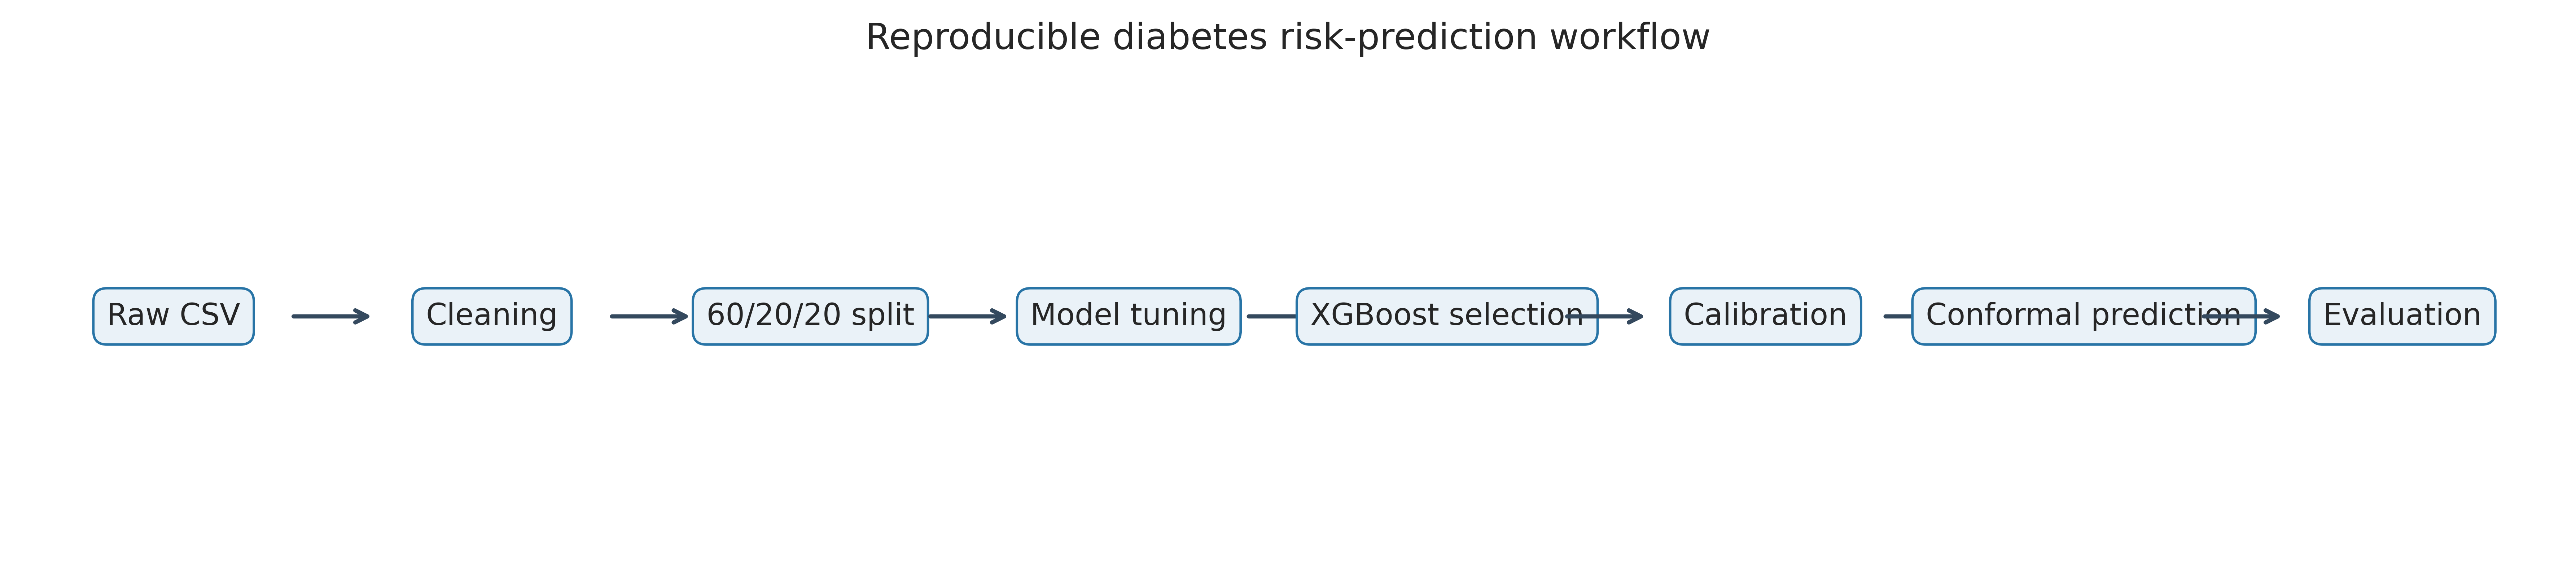
\includegraphics[width=\textwidth]{figures/figure_01_workflow_diagram_original_prevalence.png}
\caption{Reproducible primary-analysis workflow. Model tuning uses only the training partition; the held-out calibration partition is reserved for conformal scoring.}
\label{fig:workflow}
\end{figure*}

\begin{figure}[t]
\centering
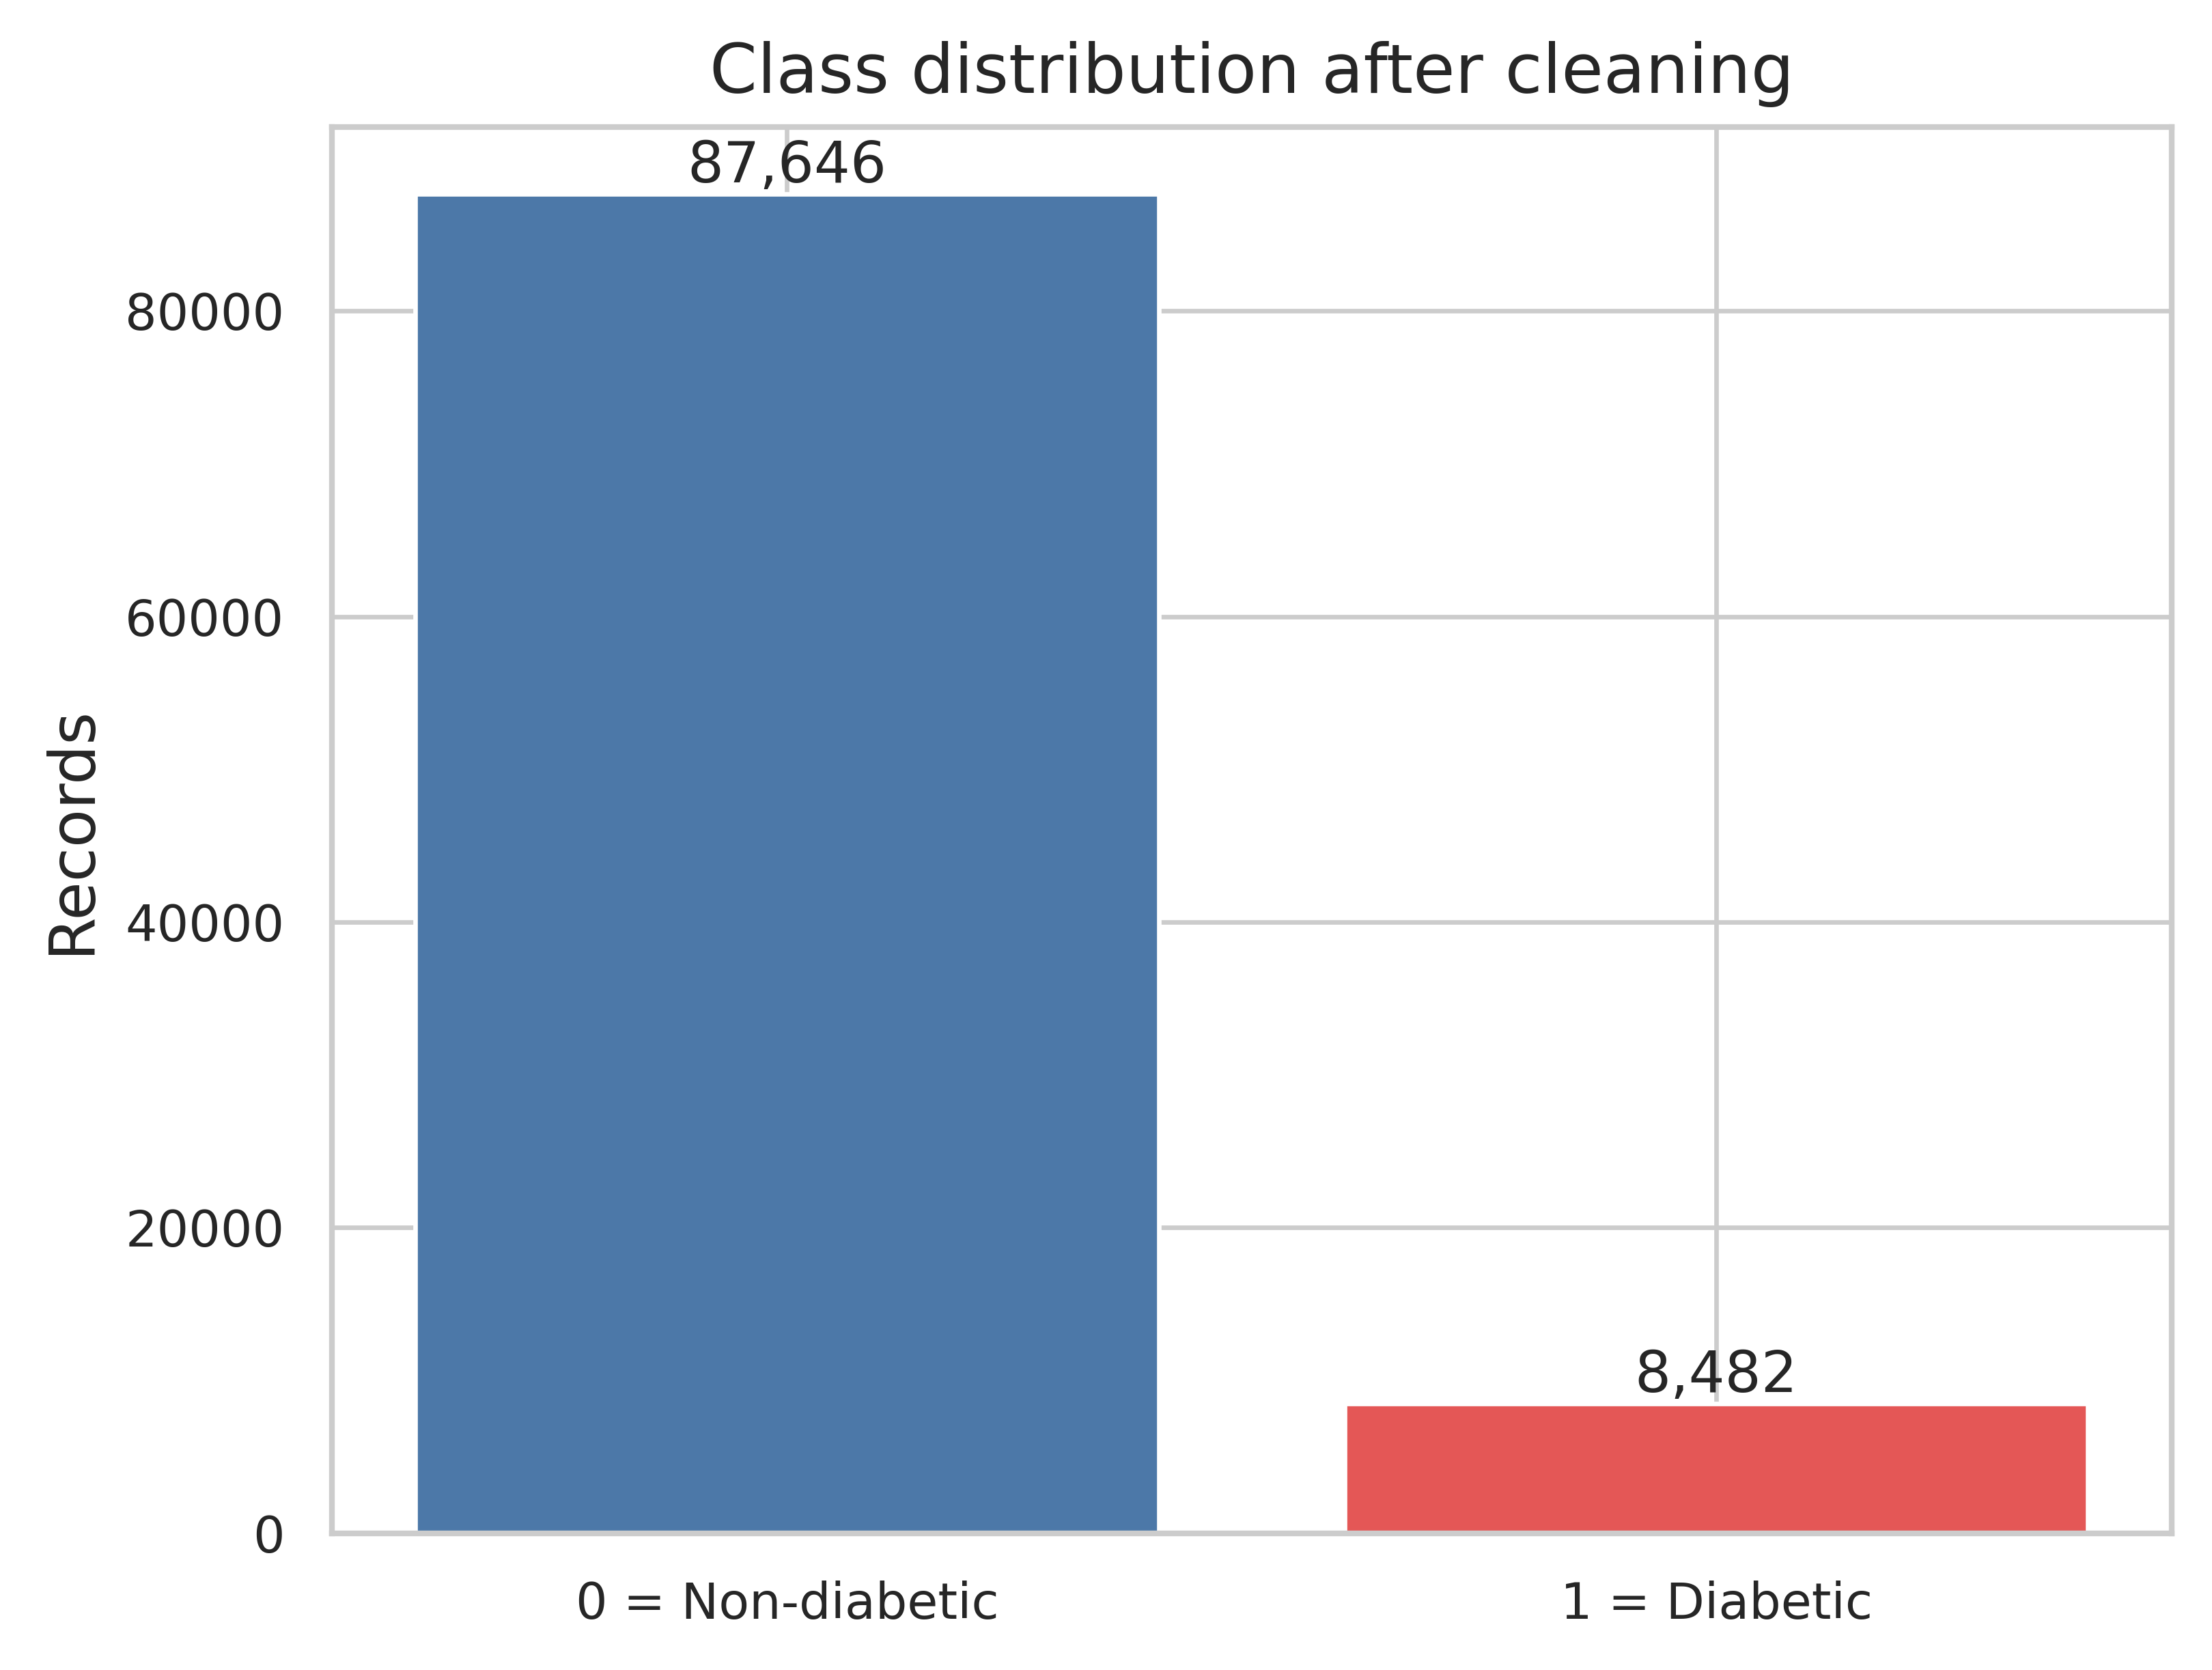
\includegraphics[width=\columnwidth]{figures/figure_02_class_distribution_original_prevalence.png}
\caption{Class distribution after data cleaning. The primary analysis retains the observed diabetes prevalence.}
\label{fig:classdistribution}
\end{figure}

\begin{table*}[t]
\caption{Test-set performance on the cleaned original-prevalence dataset. Point predictions use the calibrated probabilities and a fixed threshold of 0.5.}
\label{tab:modelcomparison}
\centering
\begin{tabular}{lrrrrrr}
\toprule
Model & Accuracy & Balanced accuracy & Sensitivity & Specificity & F1 & ROC-AUC \\
\midrule
Logistic regression & 0.8864 & 0.8815 & 0.8756 & 0.8874 & 0.5761 & 0.9595 \\
SVM & 0.9588 & 0.8120 & 0.6338 & 0.9902 & 0.7305 & 0.9584 \\
Decision tree & 0.9710 & 0.8475 & 0.6975 & 0.9975 & 0.8094 & 0.9711 \\
Random forest & 0.9041 & 0.9008 & 0.8968 & 0.9048 & 0.6226 & 0.9737 \\
XGBoost & 0.9702 & 0.8566 & 0.7188 & 0.9945 & 0.8097 & 0.9777 \\
\bottomrule
\end{tabular}
\end{table*}

XGBoost had the highest ROC-AUC (0.9777) and PR-AUC (0.8826). At threshold 0.5, it yielded 1,219 true positives, 477 false negatives, 96 false positives, and 17,434 true negatives. Its Brier score was 0.0250 and log loss was 0.0973. Bootstrap intervals showed narrow uncertainty around discrimination: ROC-AUC 0.9777 (95\% CI, 0.9751--0.9801) and PR-AUC 0.8826 (95\% CI, 0.8712--0.8932). Sensitivity was 0.7188 (95\% CI, 0.6987--0.7394), while specificity was 0.9945 (95\% CI, 0.9934--0.9955). Figure~\ref{fig:modelcomparison} compares all model families; Figs.~\ref{fig:roc}--\ref{fig:calibration} provide discrimination and calibration visualizations.

\begin{figure*}[t]
\centering
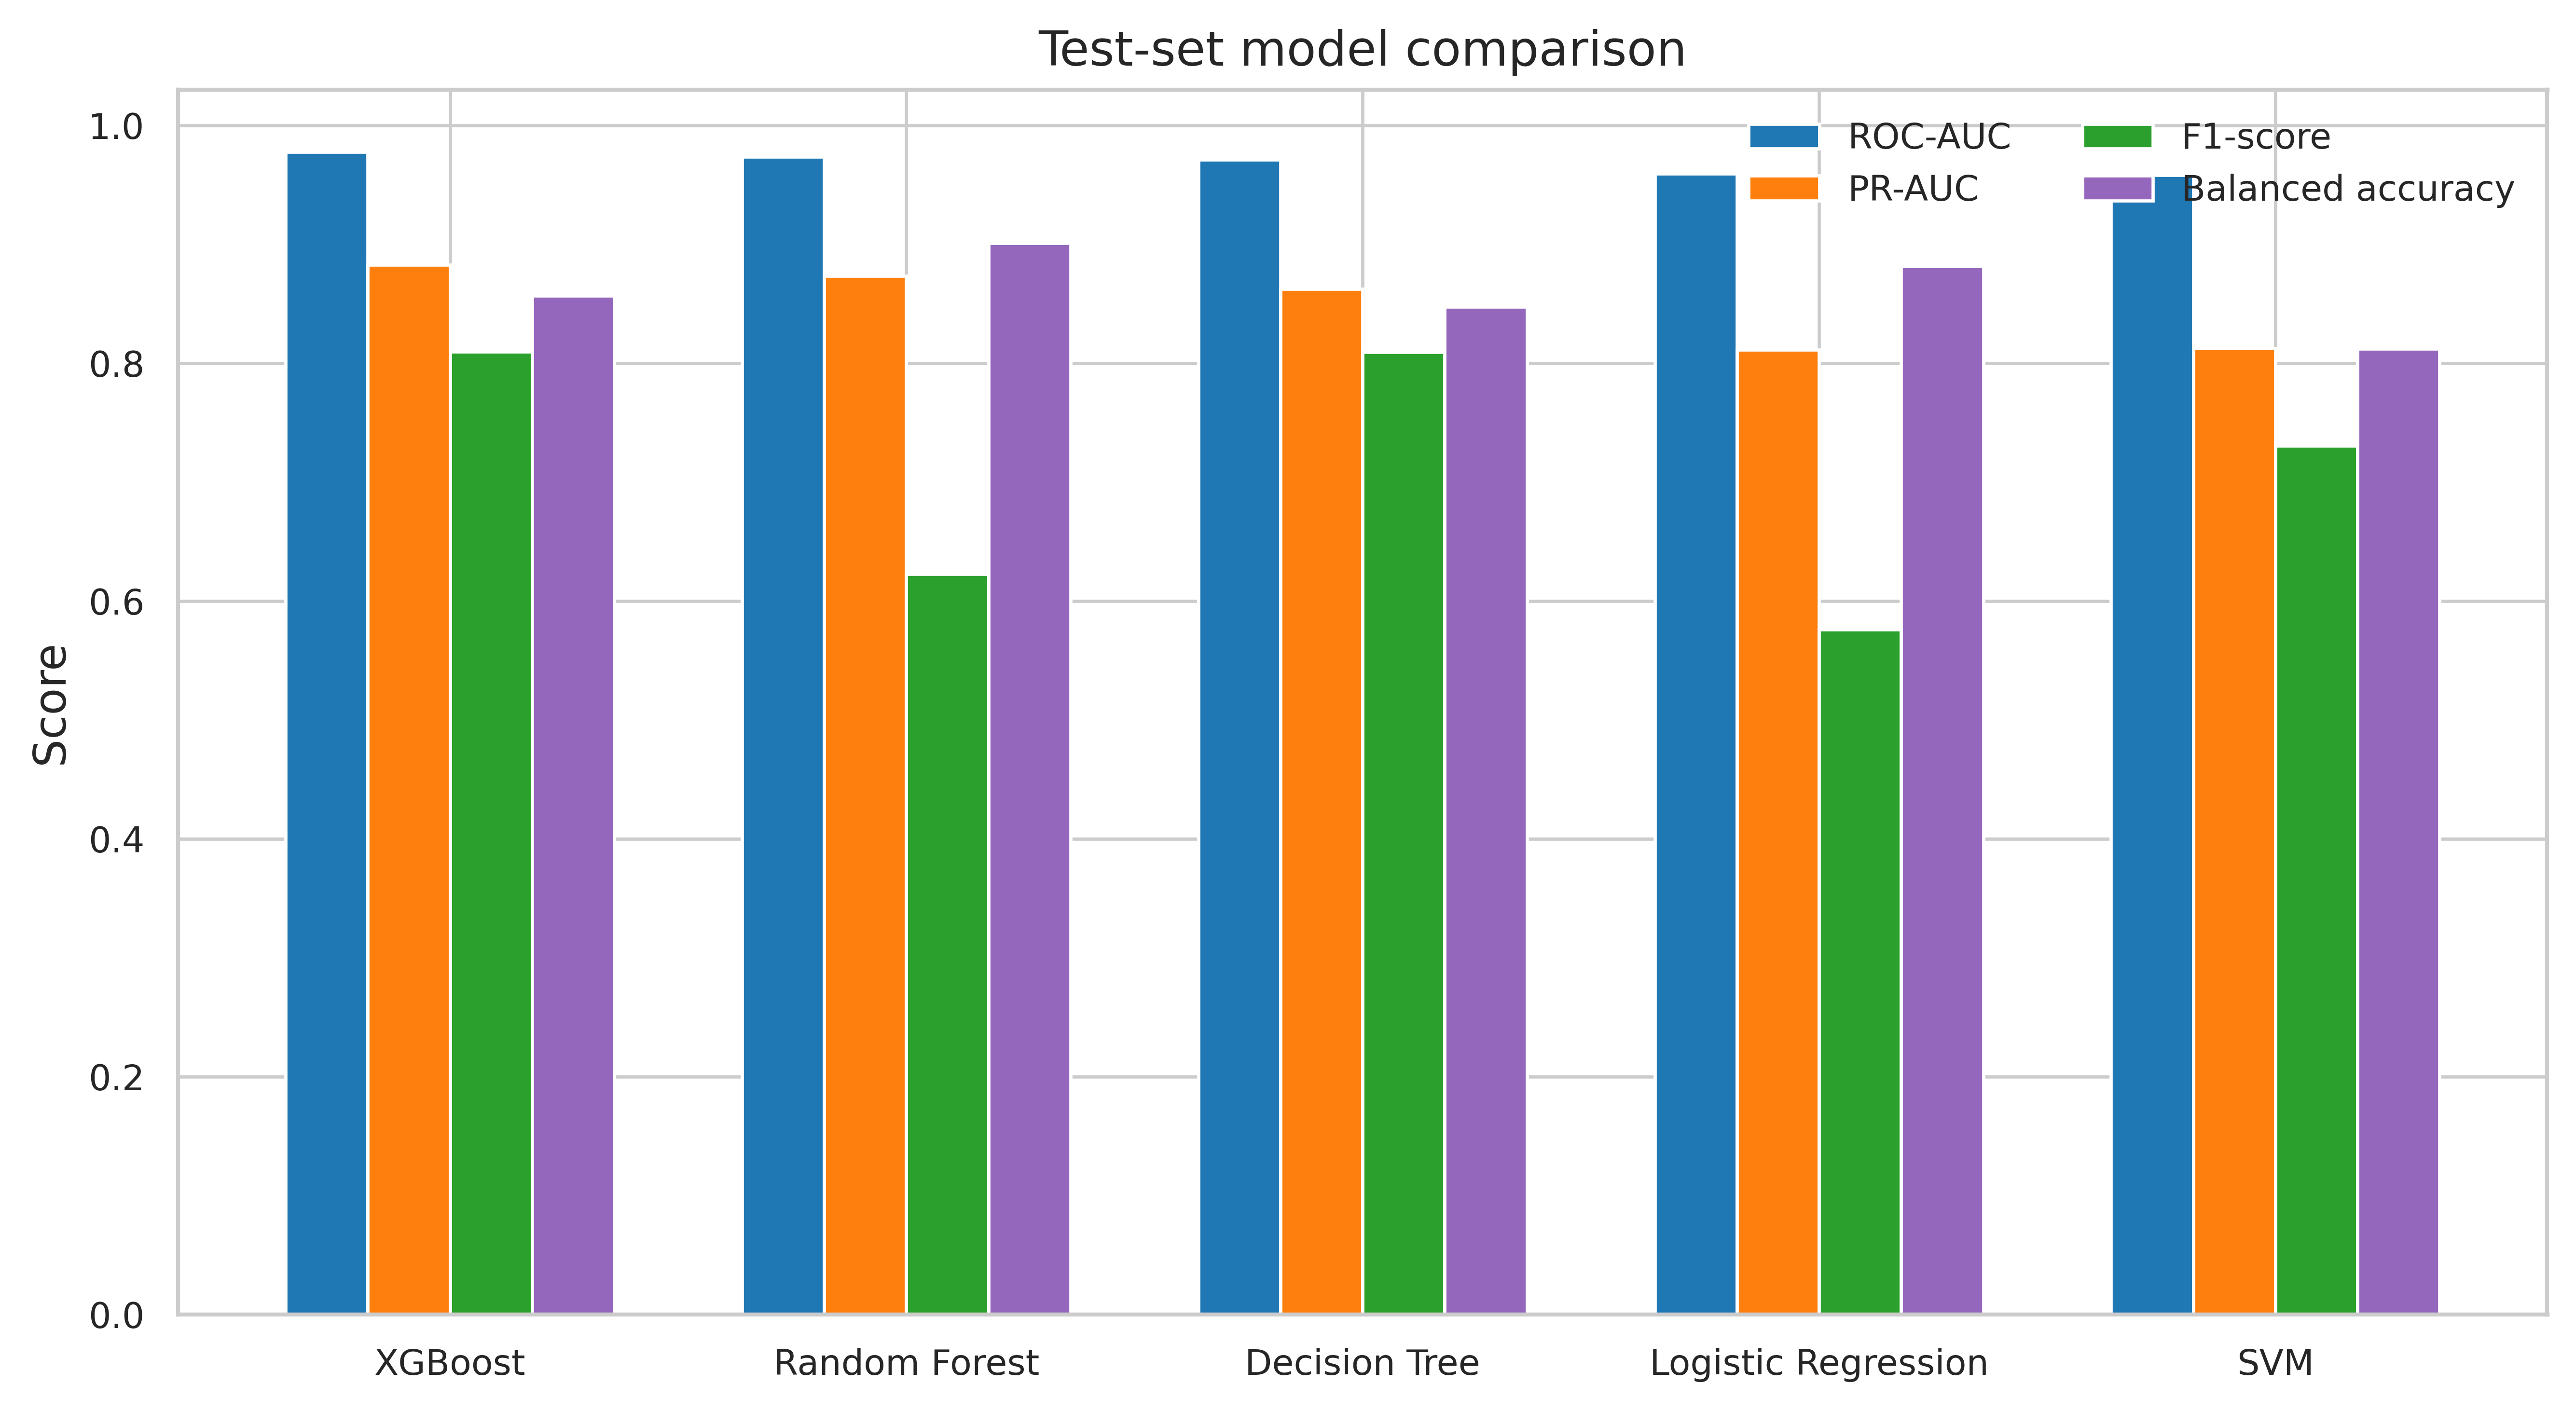
\includegraphics[width=0.72\textwidth]{figures/figure_04_model_comparison_original_prevalence.png}
\caption{Test-set comparison of tuned model families on the original-prevalence dataset.}
\label{fig:modelcomparison}
\end{figure*}

\begin{figure}[t]
\centering
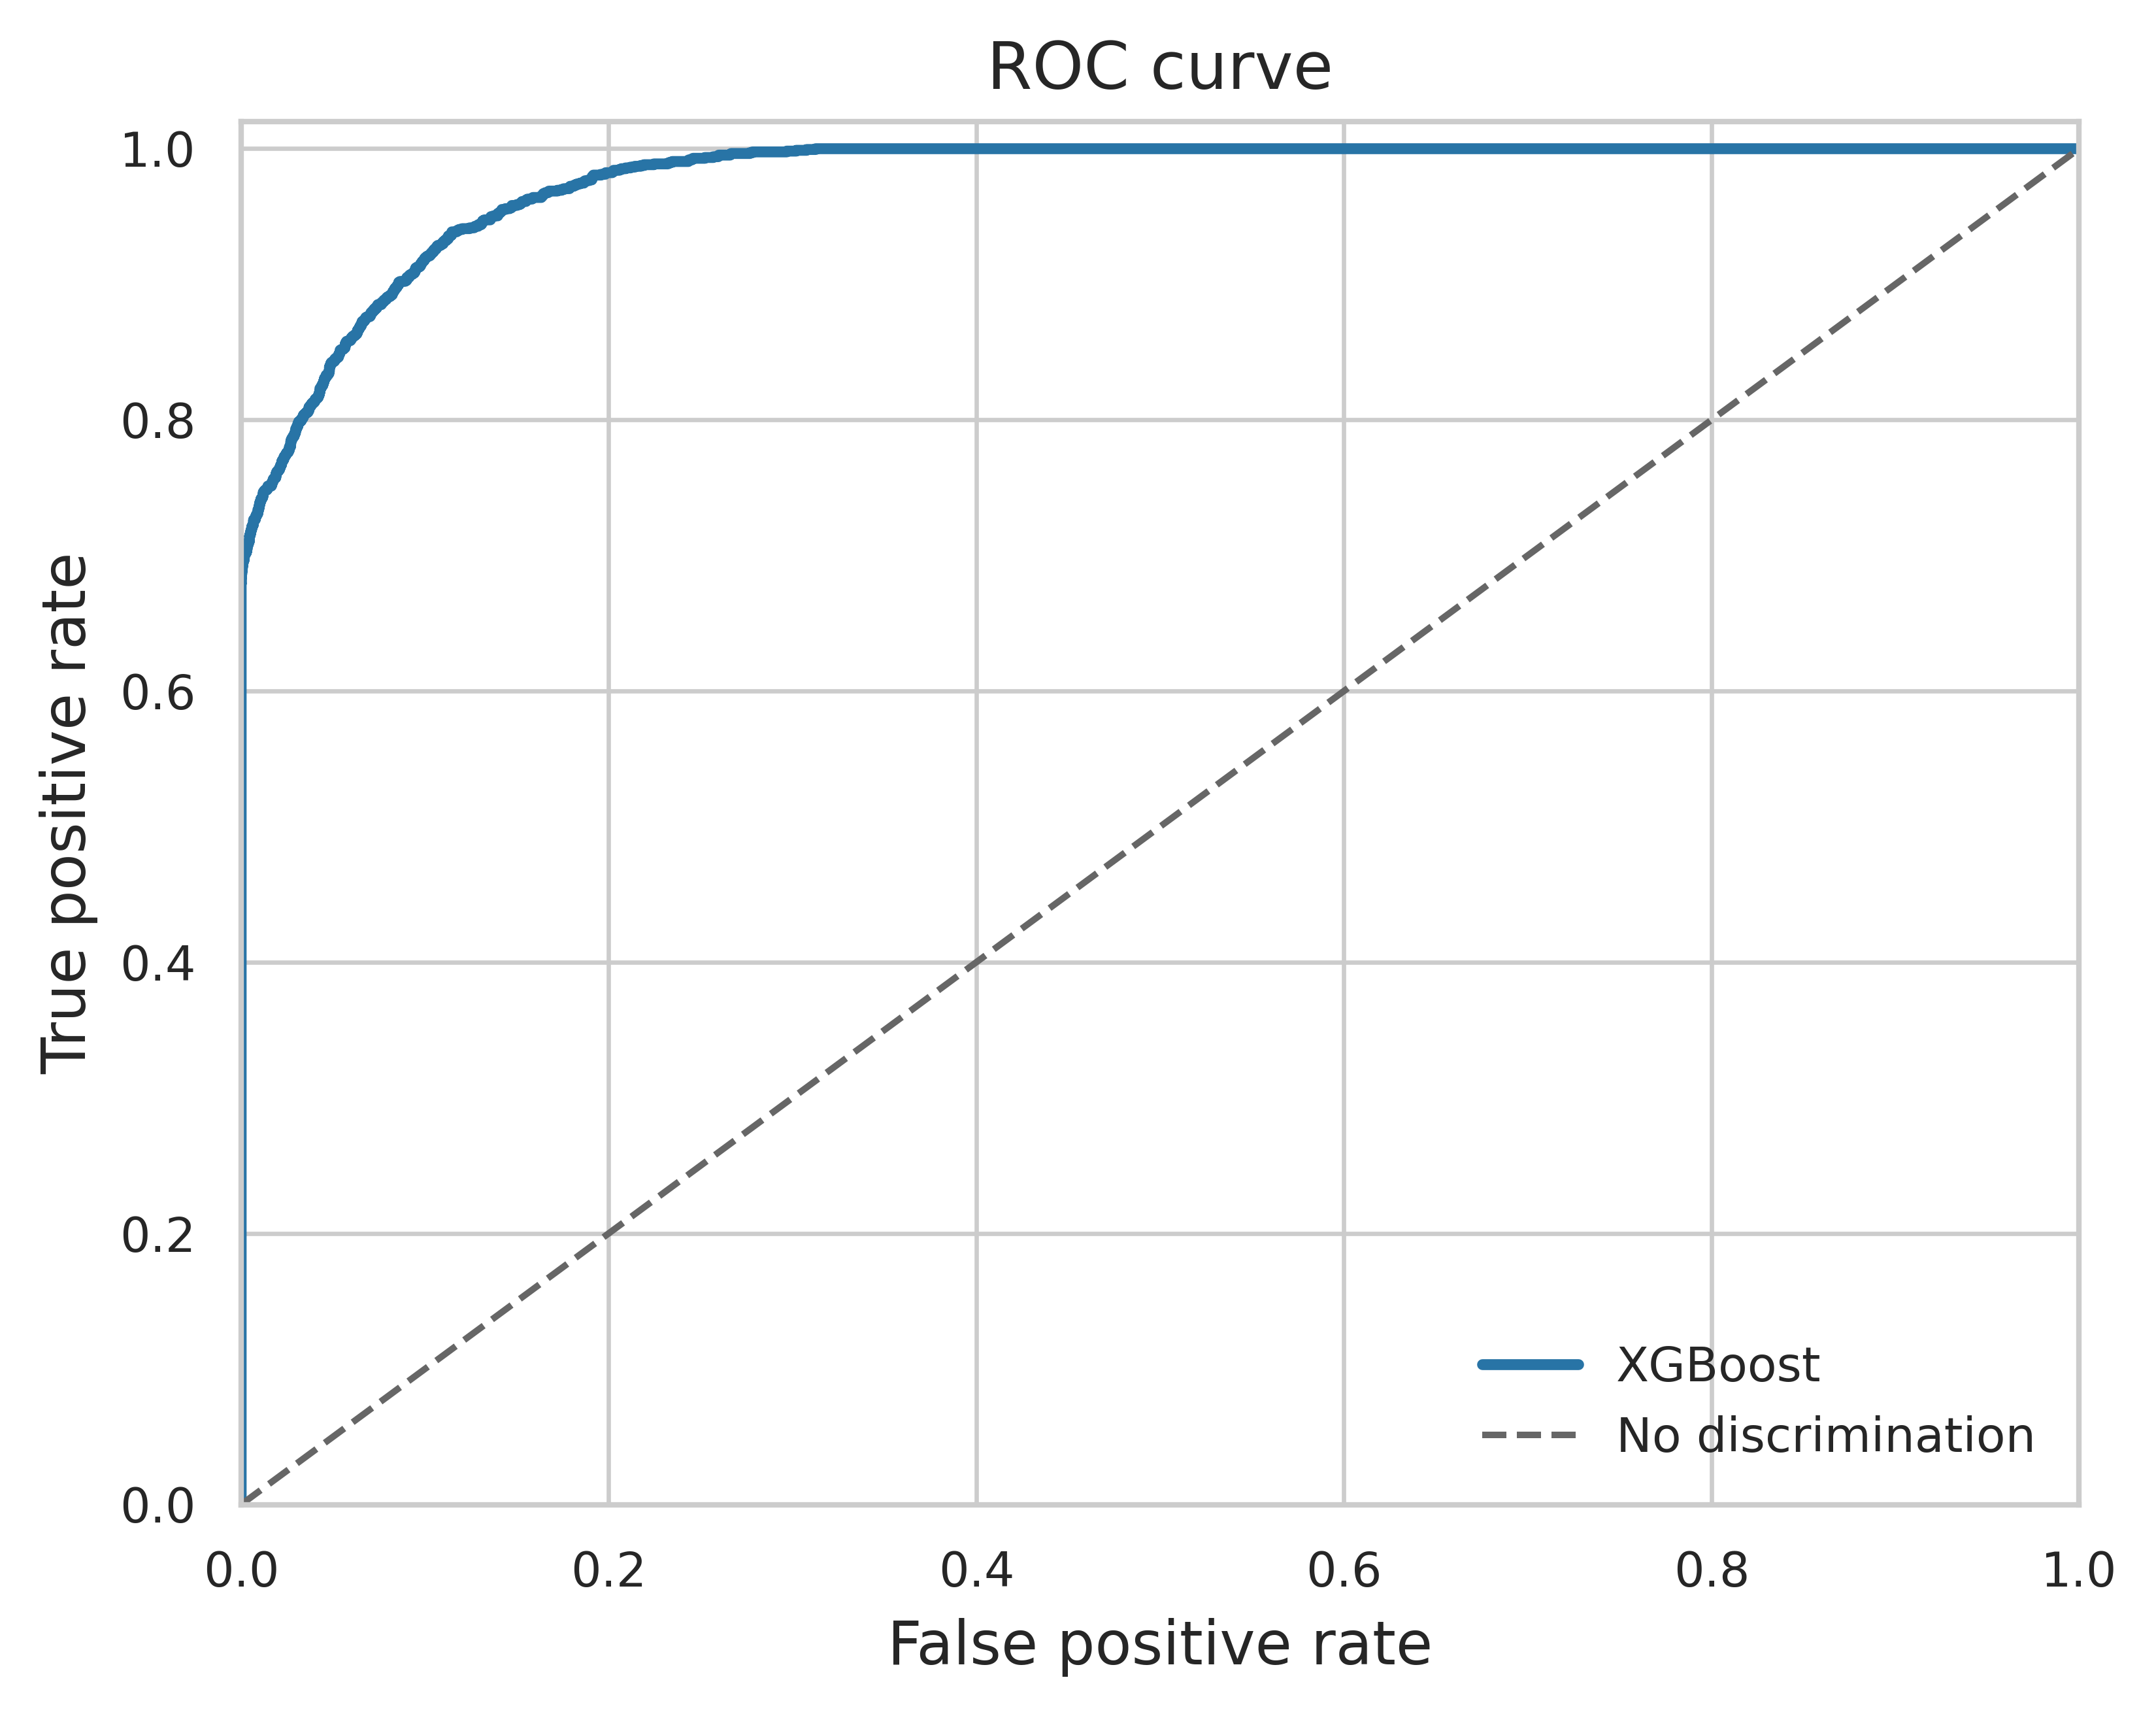
\includegraphics[width=\columnwidth]{figures/figure_06_roc_curve_original_prevalence.png}
\caption{ROC curve for calibrated XGBoost on the untouched primary test set.}
\label{fig:roc}
\end{figure}

\begin{figure}[t]
\centering
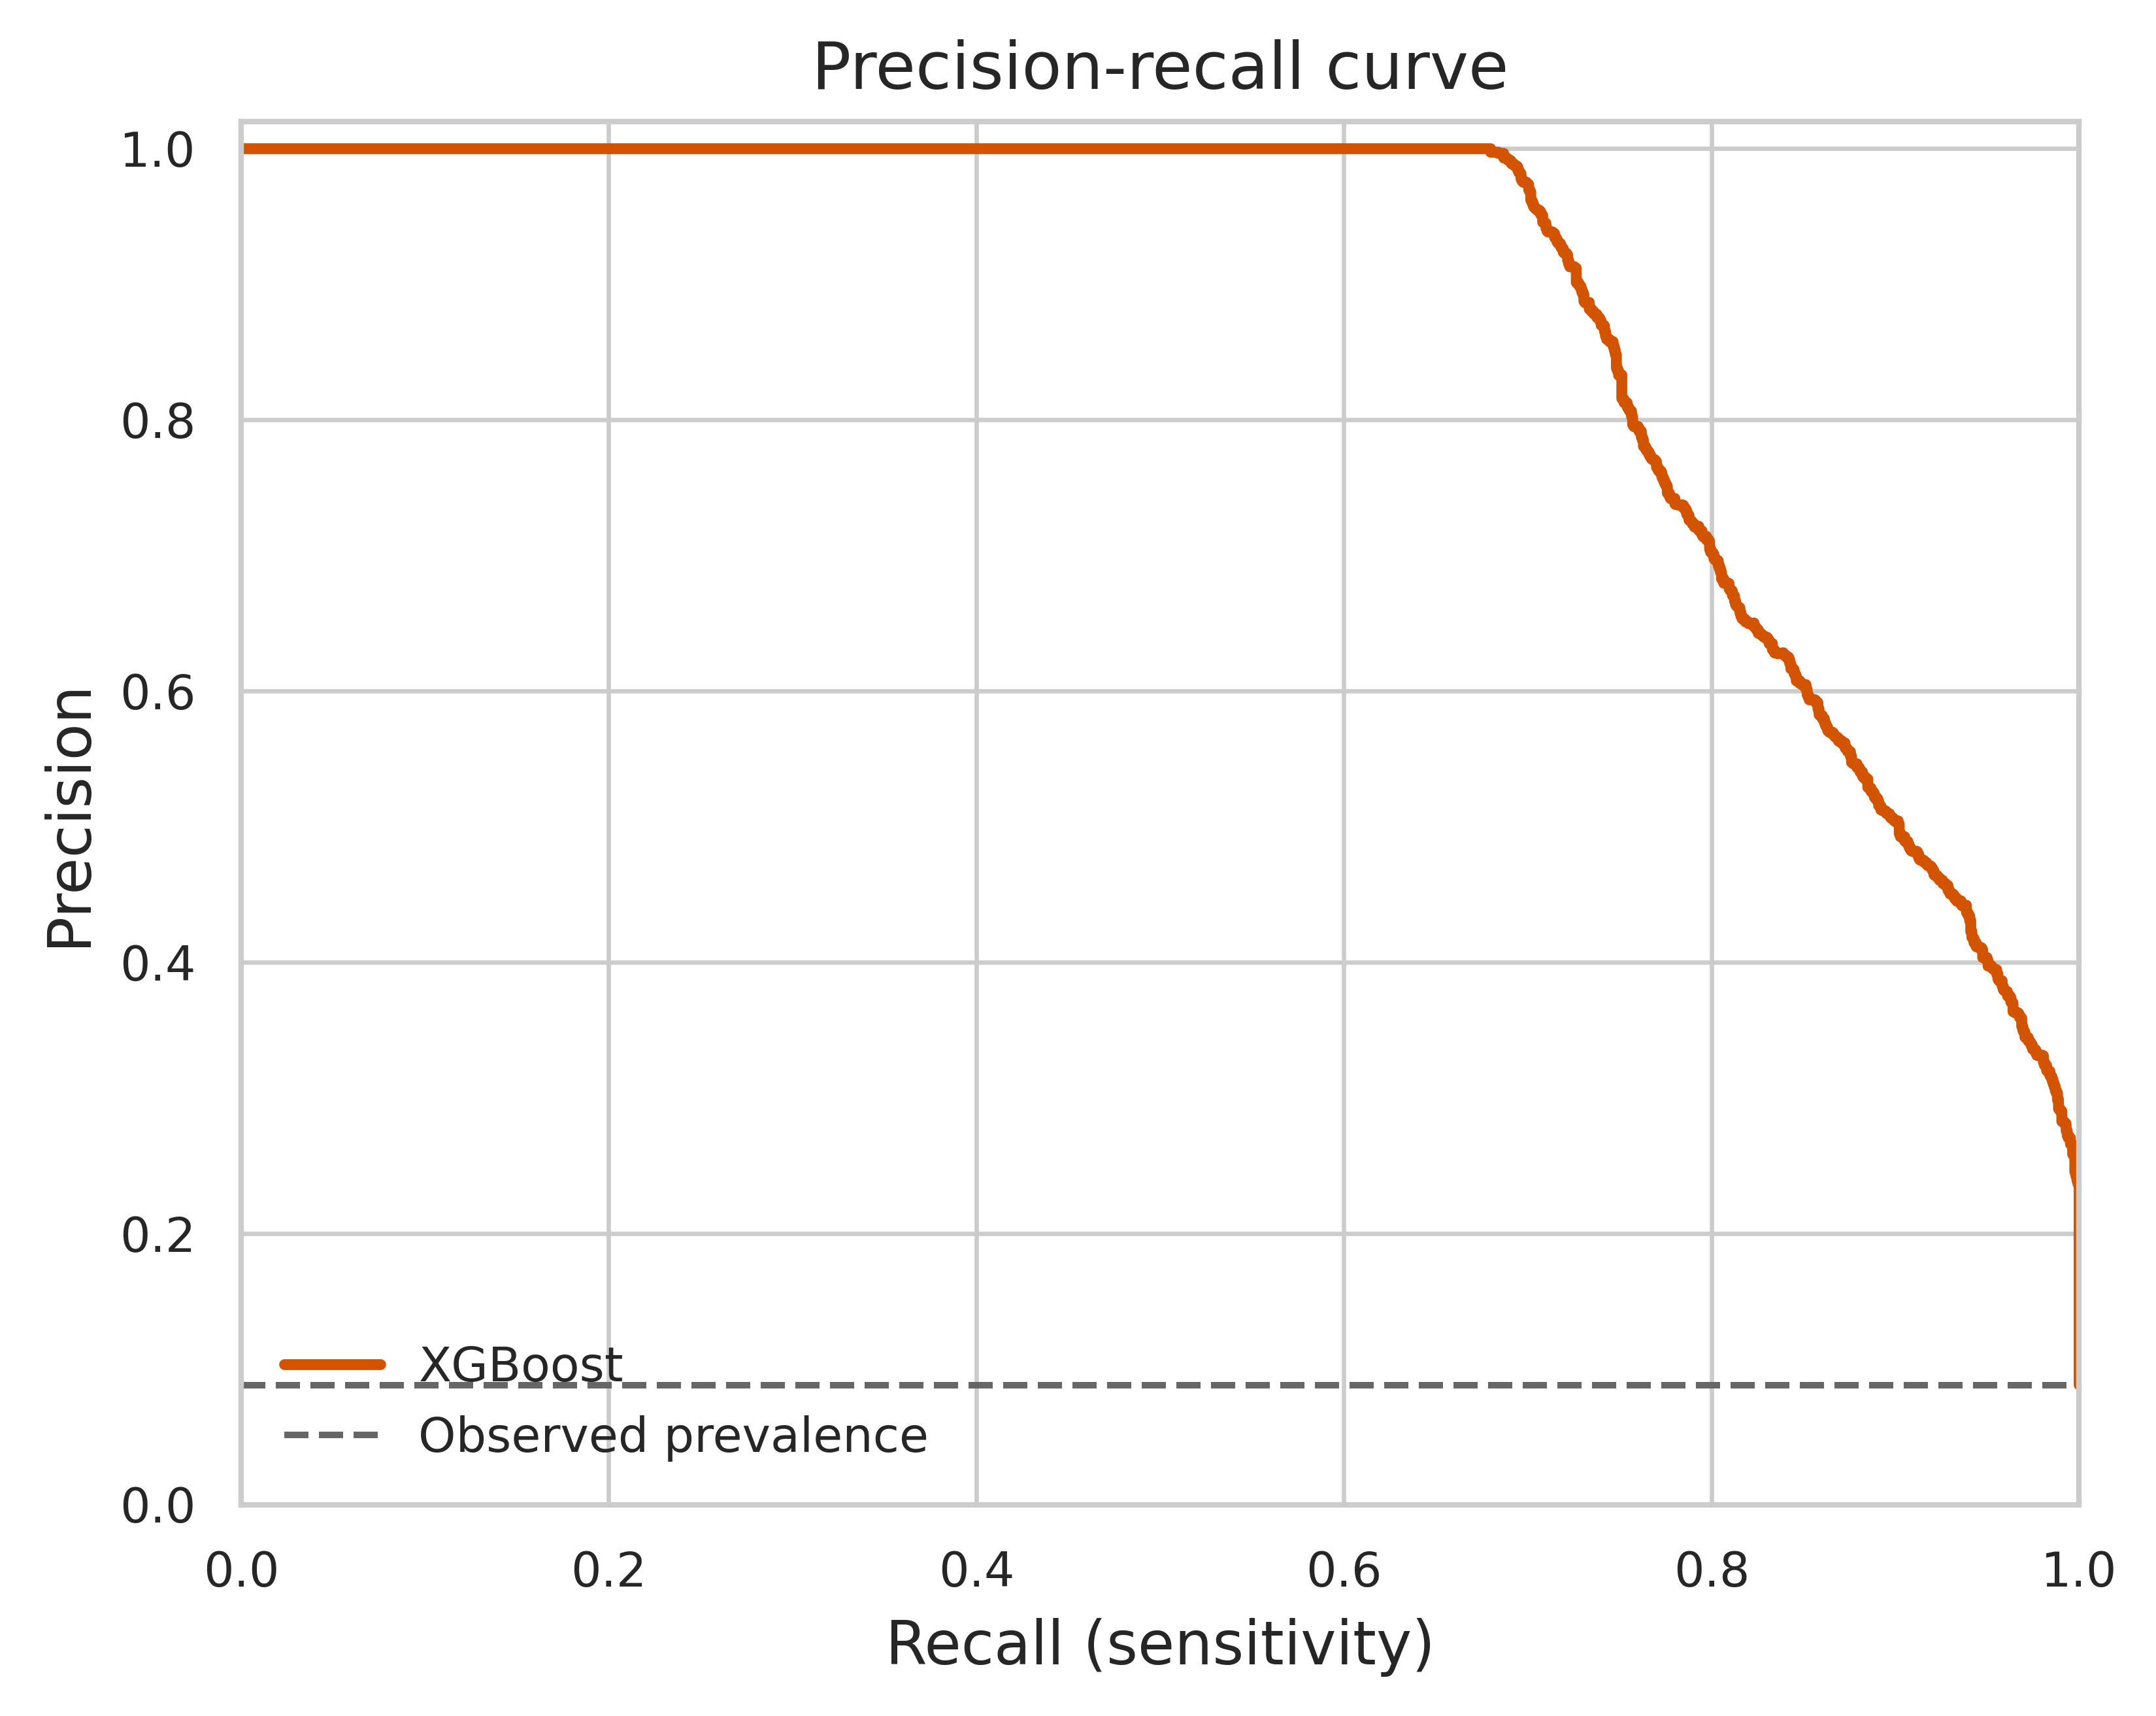
\includegraphics[width=\columnwidth]{figures/figure_07_precision_recall_curve_original_prevalence.png}
\caption{Precision--recall curve for calibrated XGBoost. The horizontal reference is the observed test prevalence.}
\label{fig:pr}
\end{figure}

\begin{figure}[t]
\centering
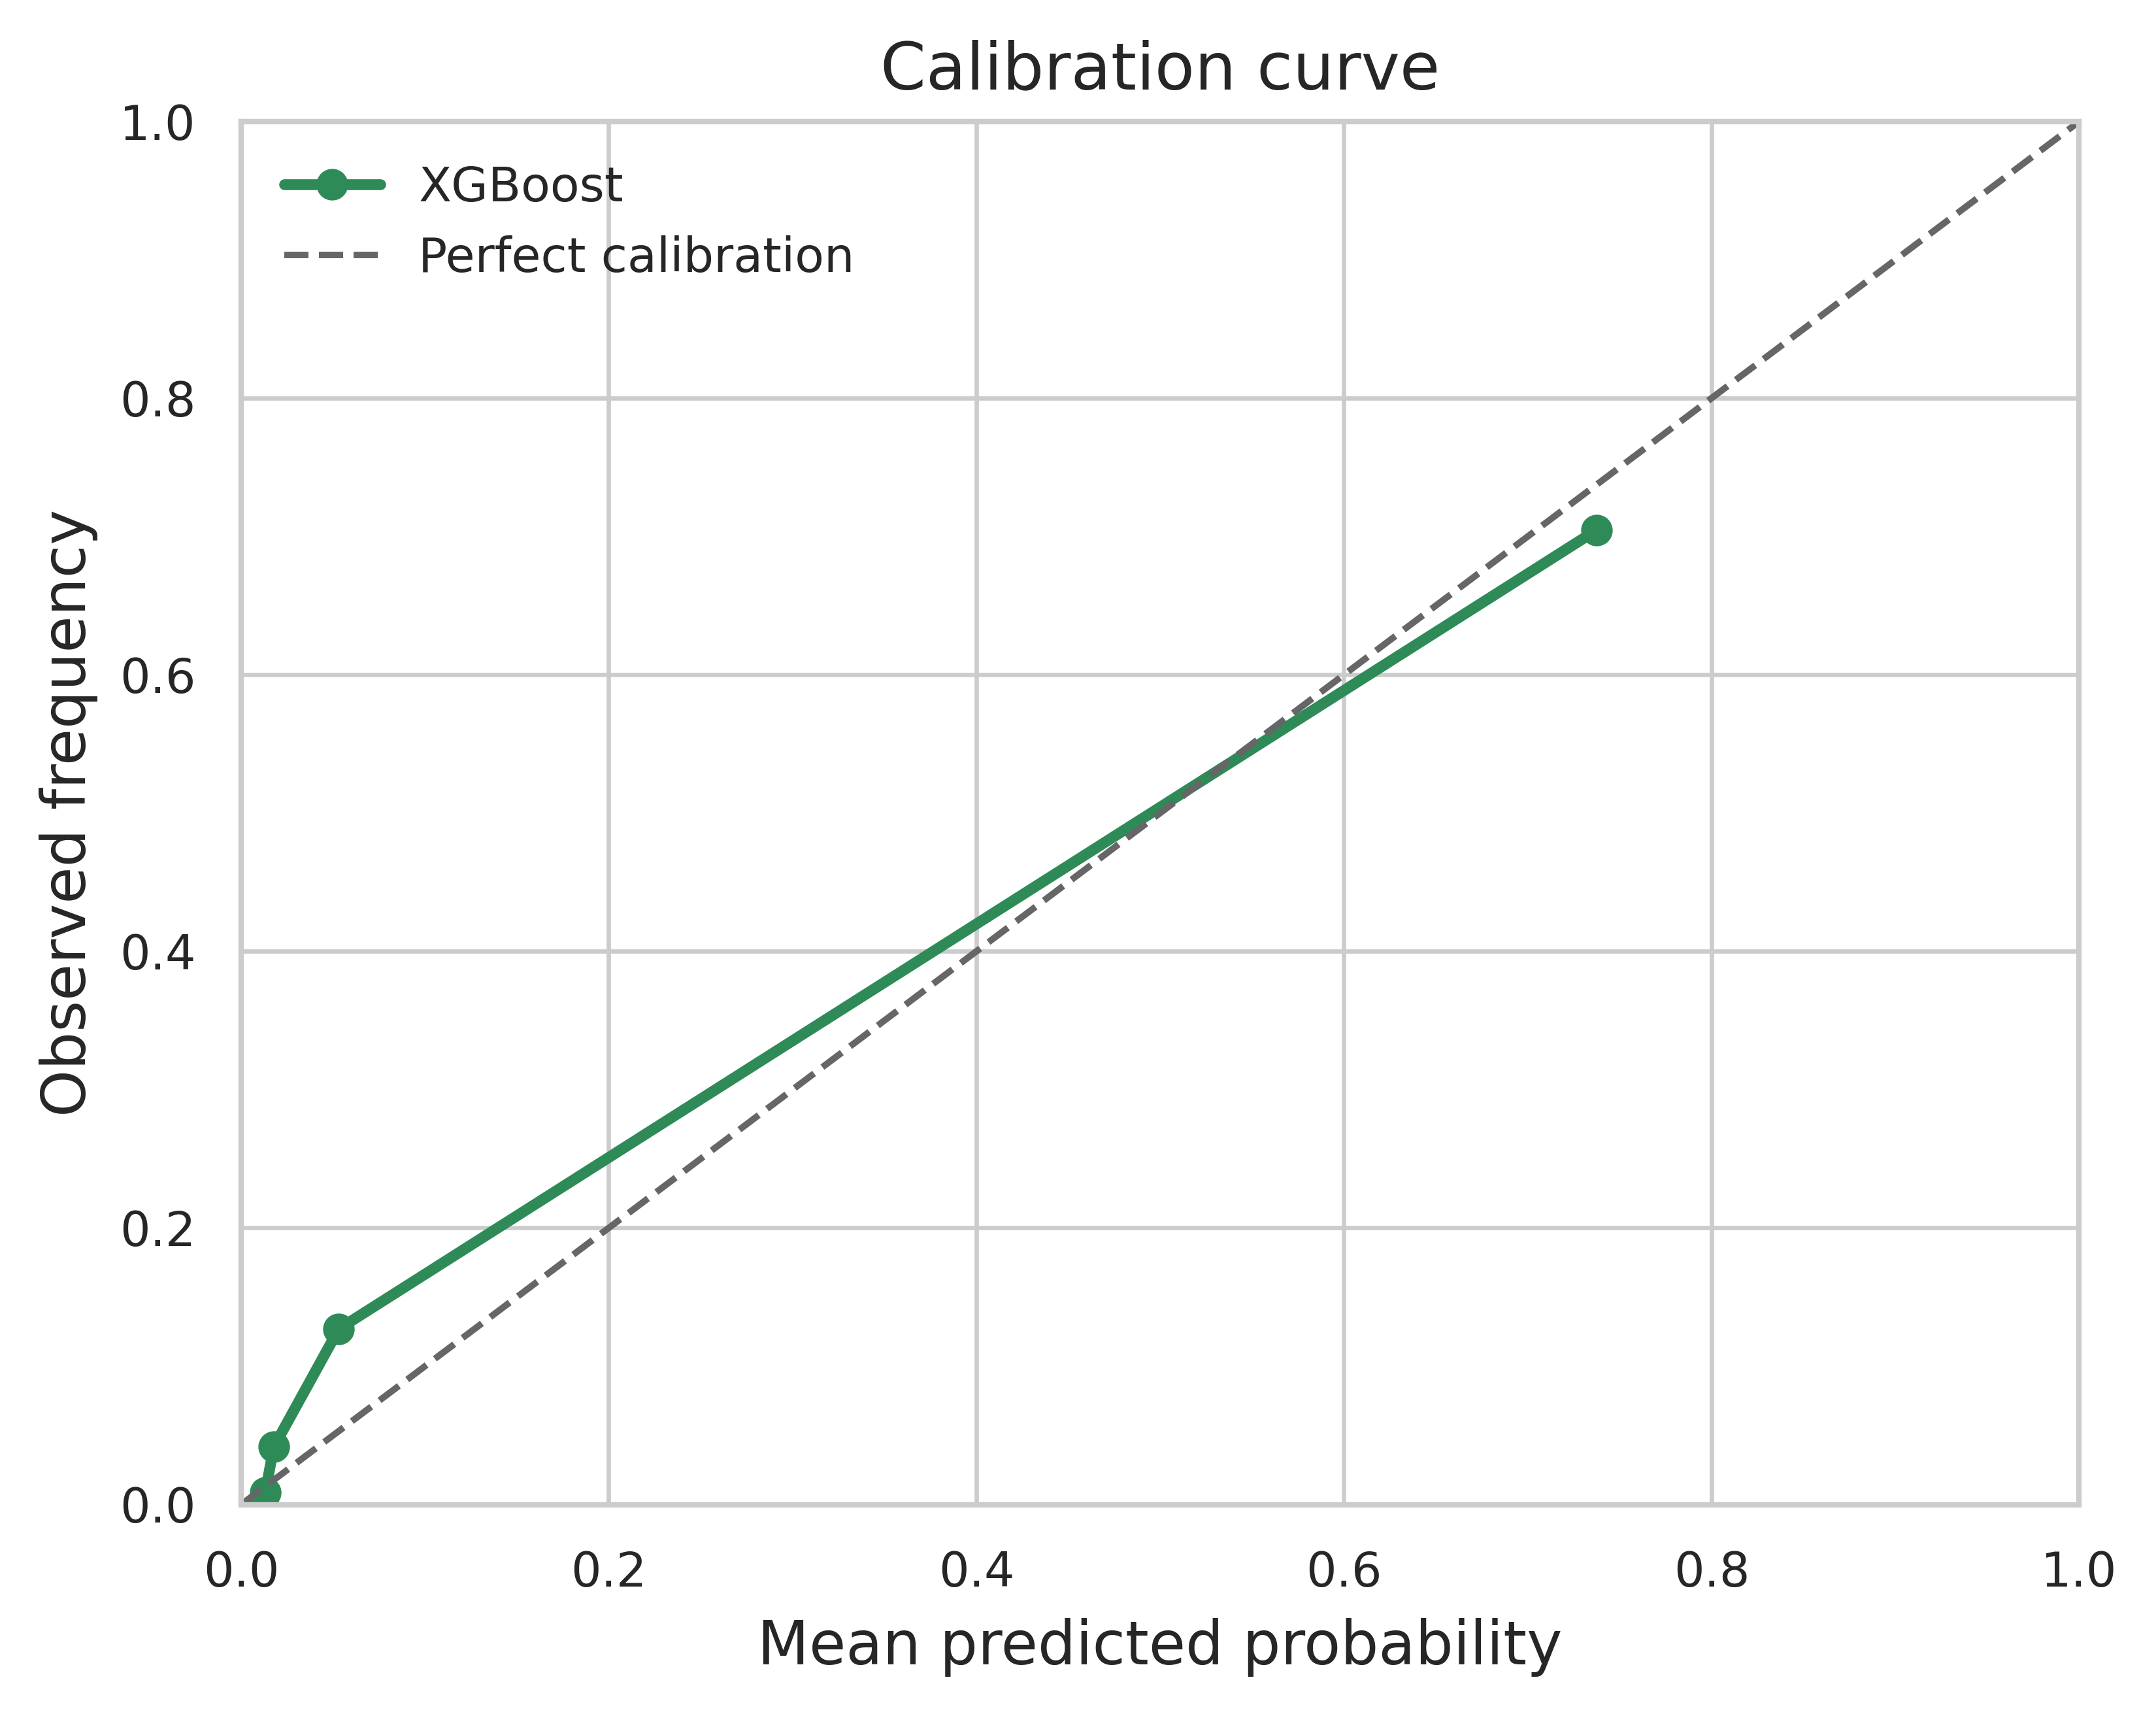
\includegraphics[width=\columnwidth]{figures/figure_08_calibration_curve_original_prevalence.png}
\caption{Reliability diagram for calibrated XGBoost on the untouched primary test set.}
\label{fig:calibration}
\end{figure}

\subsection{Operating-threshold analysis}
The threshold analysis makes the cost of emphasizing sensitivity explicit (Table~\ref{tab:thresholds}). Thresholds were selected from training-only out-of-fold probabilities; no test outcomes were used to choose them. The threshold targeting 95\% training sensitivity produced 94.10\% test sensitivity and reduced false negatives to 100, but specificity declined to 87.66\% and precision to 42.45\%. Therefore, a high-sensitivity operating point may be useful for a screening-oriented workflow only when the increased false-positive burden is acceptable. Figure~\ref{fig:threshold} visualizes this trade-off.

\begin{figure}[t]
\centering
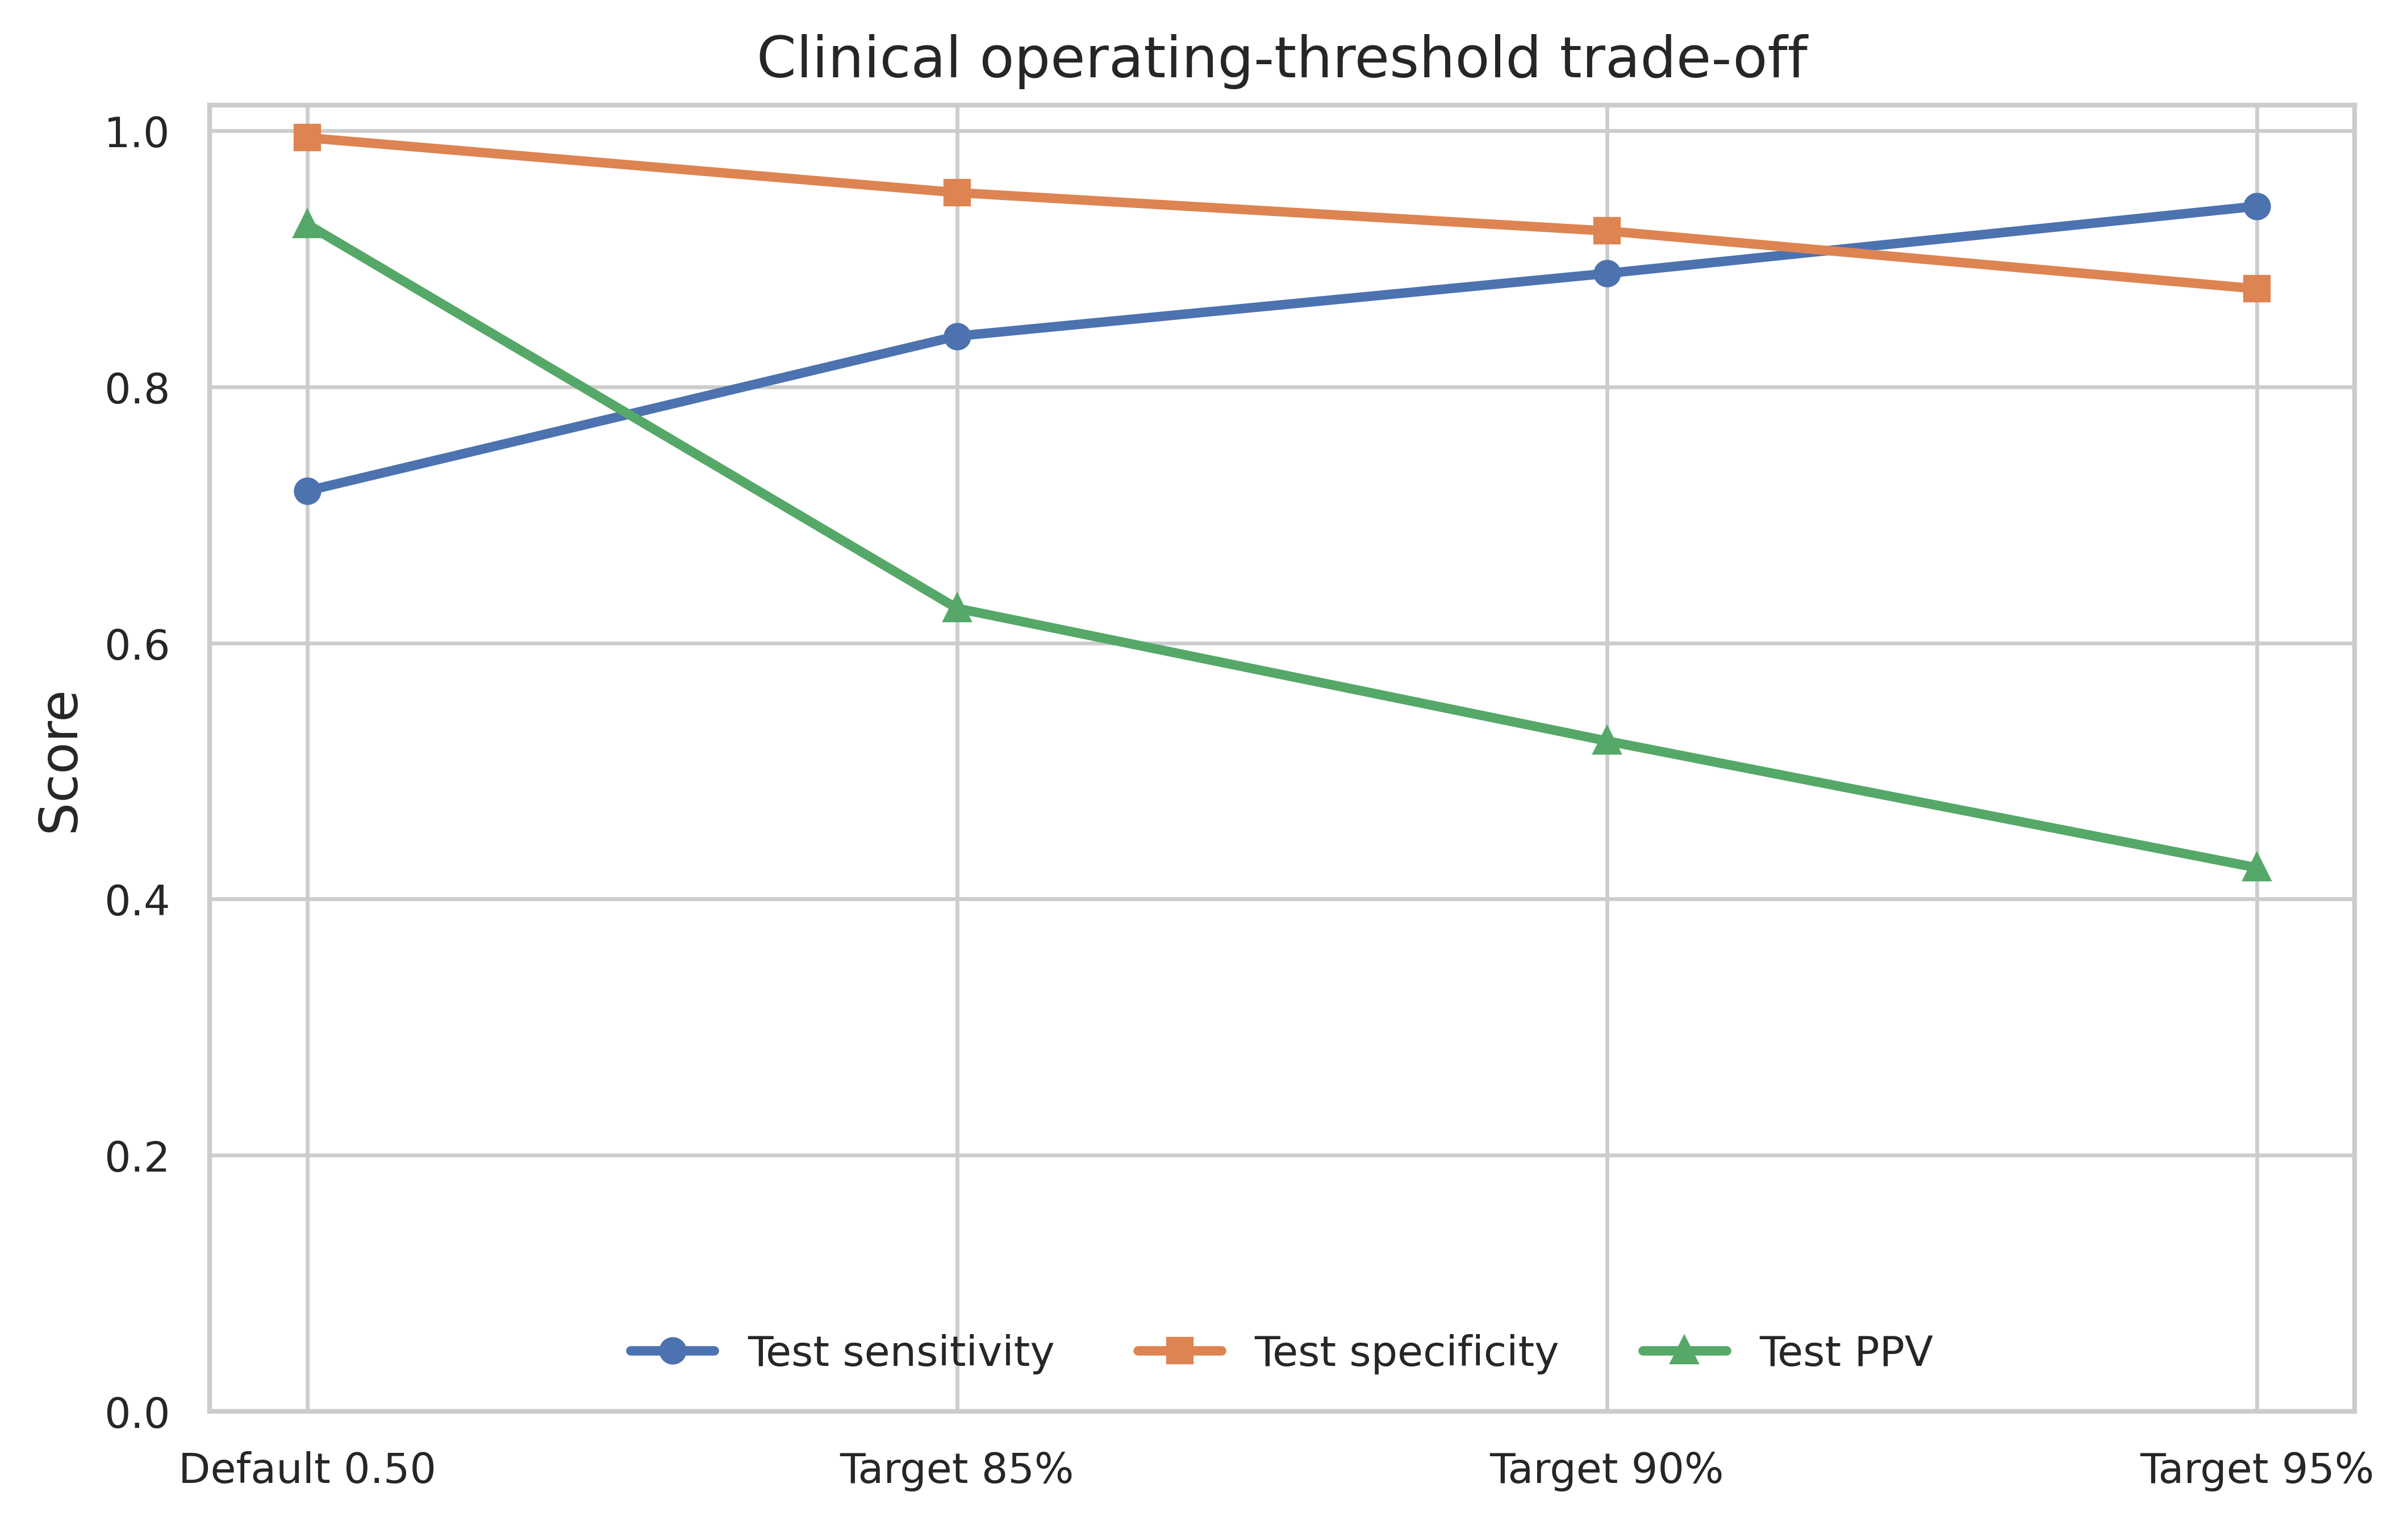
\includegraphics[width=\columnwidth]{figures/figure_16_clinical_threshold_tradeoff_original_prevalence.png}
\caption{Test-set trade-off among sensitivity, specificity, and positive predictive value at the prespecified operating points.}
\label{fig:threshold}
\end{figure}

\begin{table}[t]
\caption{Training-selected operating thresholds evaluated on the untouched test set.}
\label{tab:thresholds}
\centering
\begin{tabular}{lrrrrr}
\toprule
Target sensitivity & Threshold & Sensitivity & Specificity & PPV & FN \\
\midrule
Default 0.5 & 0.5000 & 0.7188 & 0.9945 & 0.9270 & 477 \\
85\% & 0.0788 & 0.8396 & 0.9517 & 0.6270 & 272 \\
90\% & 0.0442 & 0.8886 & 0.9217 & 0.5234 & 189 \\
95\% & 0.0253 & 0.9410 & 0.8766 & 0.4245 & 100 \\
\bottomrule
\end{tabular}
\end{table}

\subsection{Conformal reliability}
Standard split conformal prediction achieved marginal coverage close to nominal levels, but it did not provide adequate class-1 coverage. At 90\% confidence, marginal coverage was 89.84\%, class-0 coverage was 91.94\%, and class-1 coverage was 68.10\%. This difference illustrates why marginal coverage alone is insufficient for the present class-imbalanced setting.

Mondrian conformal prediction substantially improved class-wise alignment with the nominal confidence level (Table~\ref{tab:conformal}). At 90\% confidence, class-0 and class-1 coverages were 89.73\% and 89.98\%, respectively. At 95\% confidence, corresponding coverages were 94.84\% and 94.93\%. The improvement required larger prediction sets: at 95\% confidence, the mean set size was 1.086 and 8.60\% of test records received a doubleton set. This behavior is desirable to report because it represents explicit uncertainty rather than hidden misclassification. Figure~\ref{fig:conformalcomparison} compares both procedures.

\begin{figure*}[t]
\centering
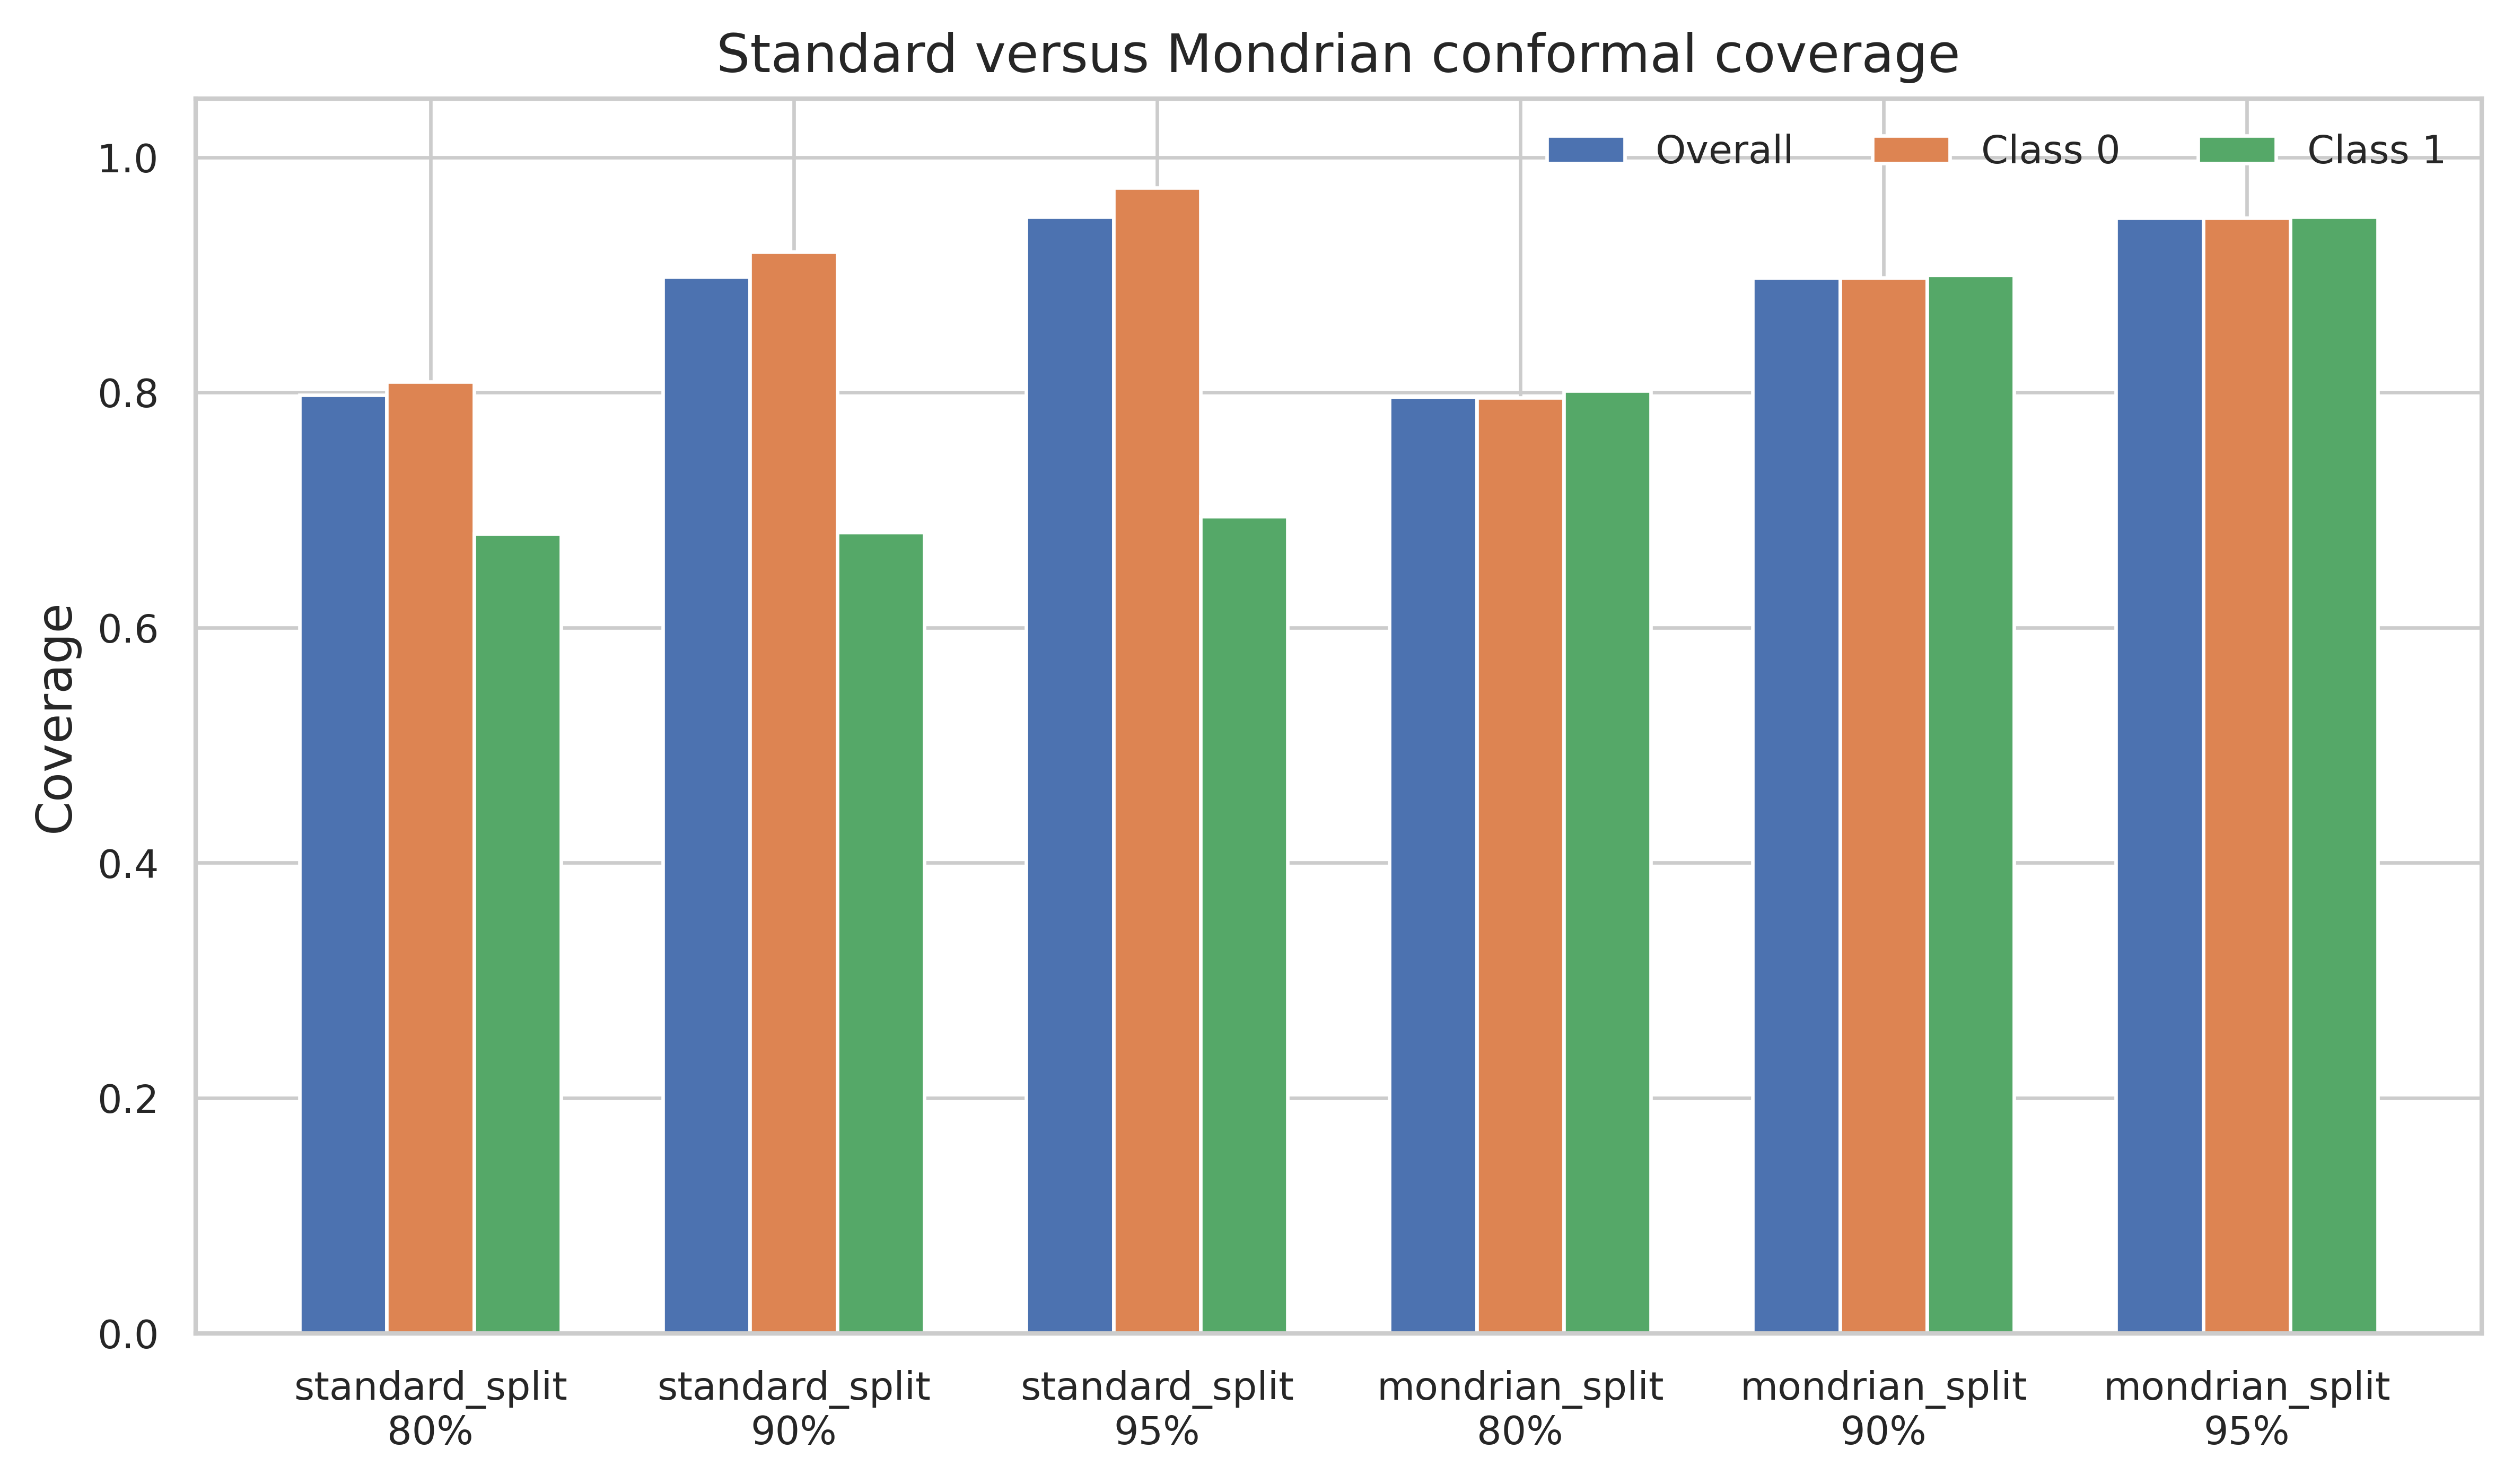
\includegraphics[width=0.78\textwidth]{figures/figure_17_conformal_method_comparison_original_prevalence.png}
\caption{Overall and class-wise empirical coverage for standard and Mondrian conformal prediction.}
\label{fig:conformalcomparison}
\end{figure*}

\begin{table*}[t]
\caption{Comparison of standard and Mondrian conformal prediction on the primary test set. Coverage is the proportion of records for which the observed label is in the prediction set.}
\label{tab:conformal}
\centering
\begin{tabular}{llrrrrrr}
\toprule
Method & Confidence & Overall coverage & Class-0 coverage & Class-1 coverage & Mean set size & Doubleton rate & Empty-set rate \\
\midrule
Standard split & 80\% & 0.7978 & 0.8092 & 0.6798 & 0.7999 & 0.0000 & 0.2001 \\
Standard split & 90\% & 0.8984 & 0.9194 & 0.6810 & 0.9081 & 0.0000 & 0.0919 \\
Standard split & 95\% & 0.9494 & 0.9740 & 0.6946 & 0.9699 & 0.0000 & 0.0301 \\
Mondrian split & 80\% & 0.7962 & 0.7957 & 0.8013 & 0.8278 & 0.0000 & 0.1722 \\
Mondrian split & 90\% & 0.8975 & 0.8973 & 0.8998 & 0.9825 & 0.0000 & 0.0175 \\
Mondrian split & 95\% & 0.9485 & 0.9484 & 0.9493 & 1.0860 & 0.0860 & 0.0000 \\
\bottomrule
\end{tabular}
\end{table*}

Calibration-size sensitivity indicated stable marginal coverage across calibration fractions. For standard split conformal prediction, mean coverage using 10\% of the calibration set was 0.7970, 0.8962, and 0.9490 at nominal 80\%, 90\%, and 95\% confidence, respectively. Variability decreased as the calibration fraction increased (Fig.~\ref{fig:calsize}).

\begin{figure}[t]
\centering
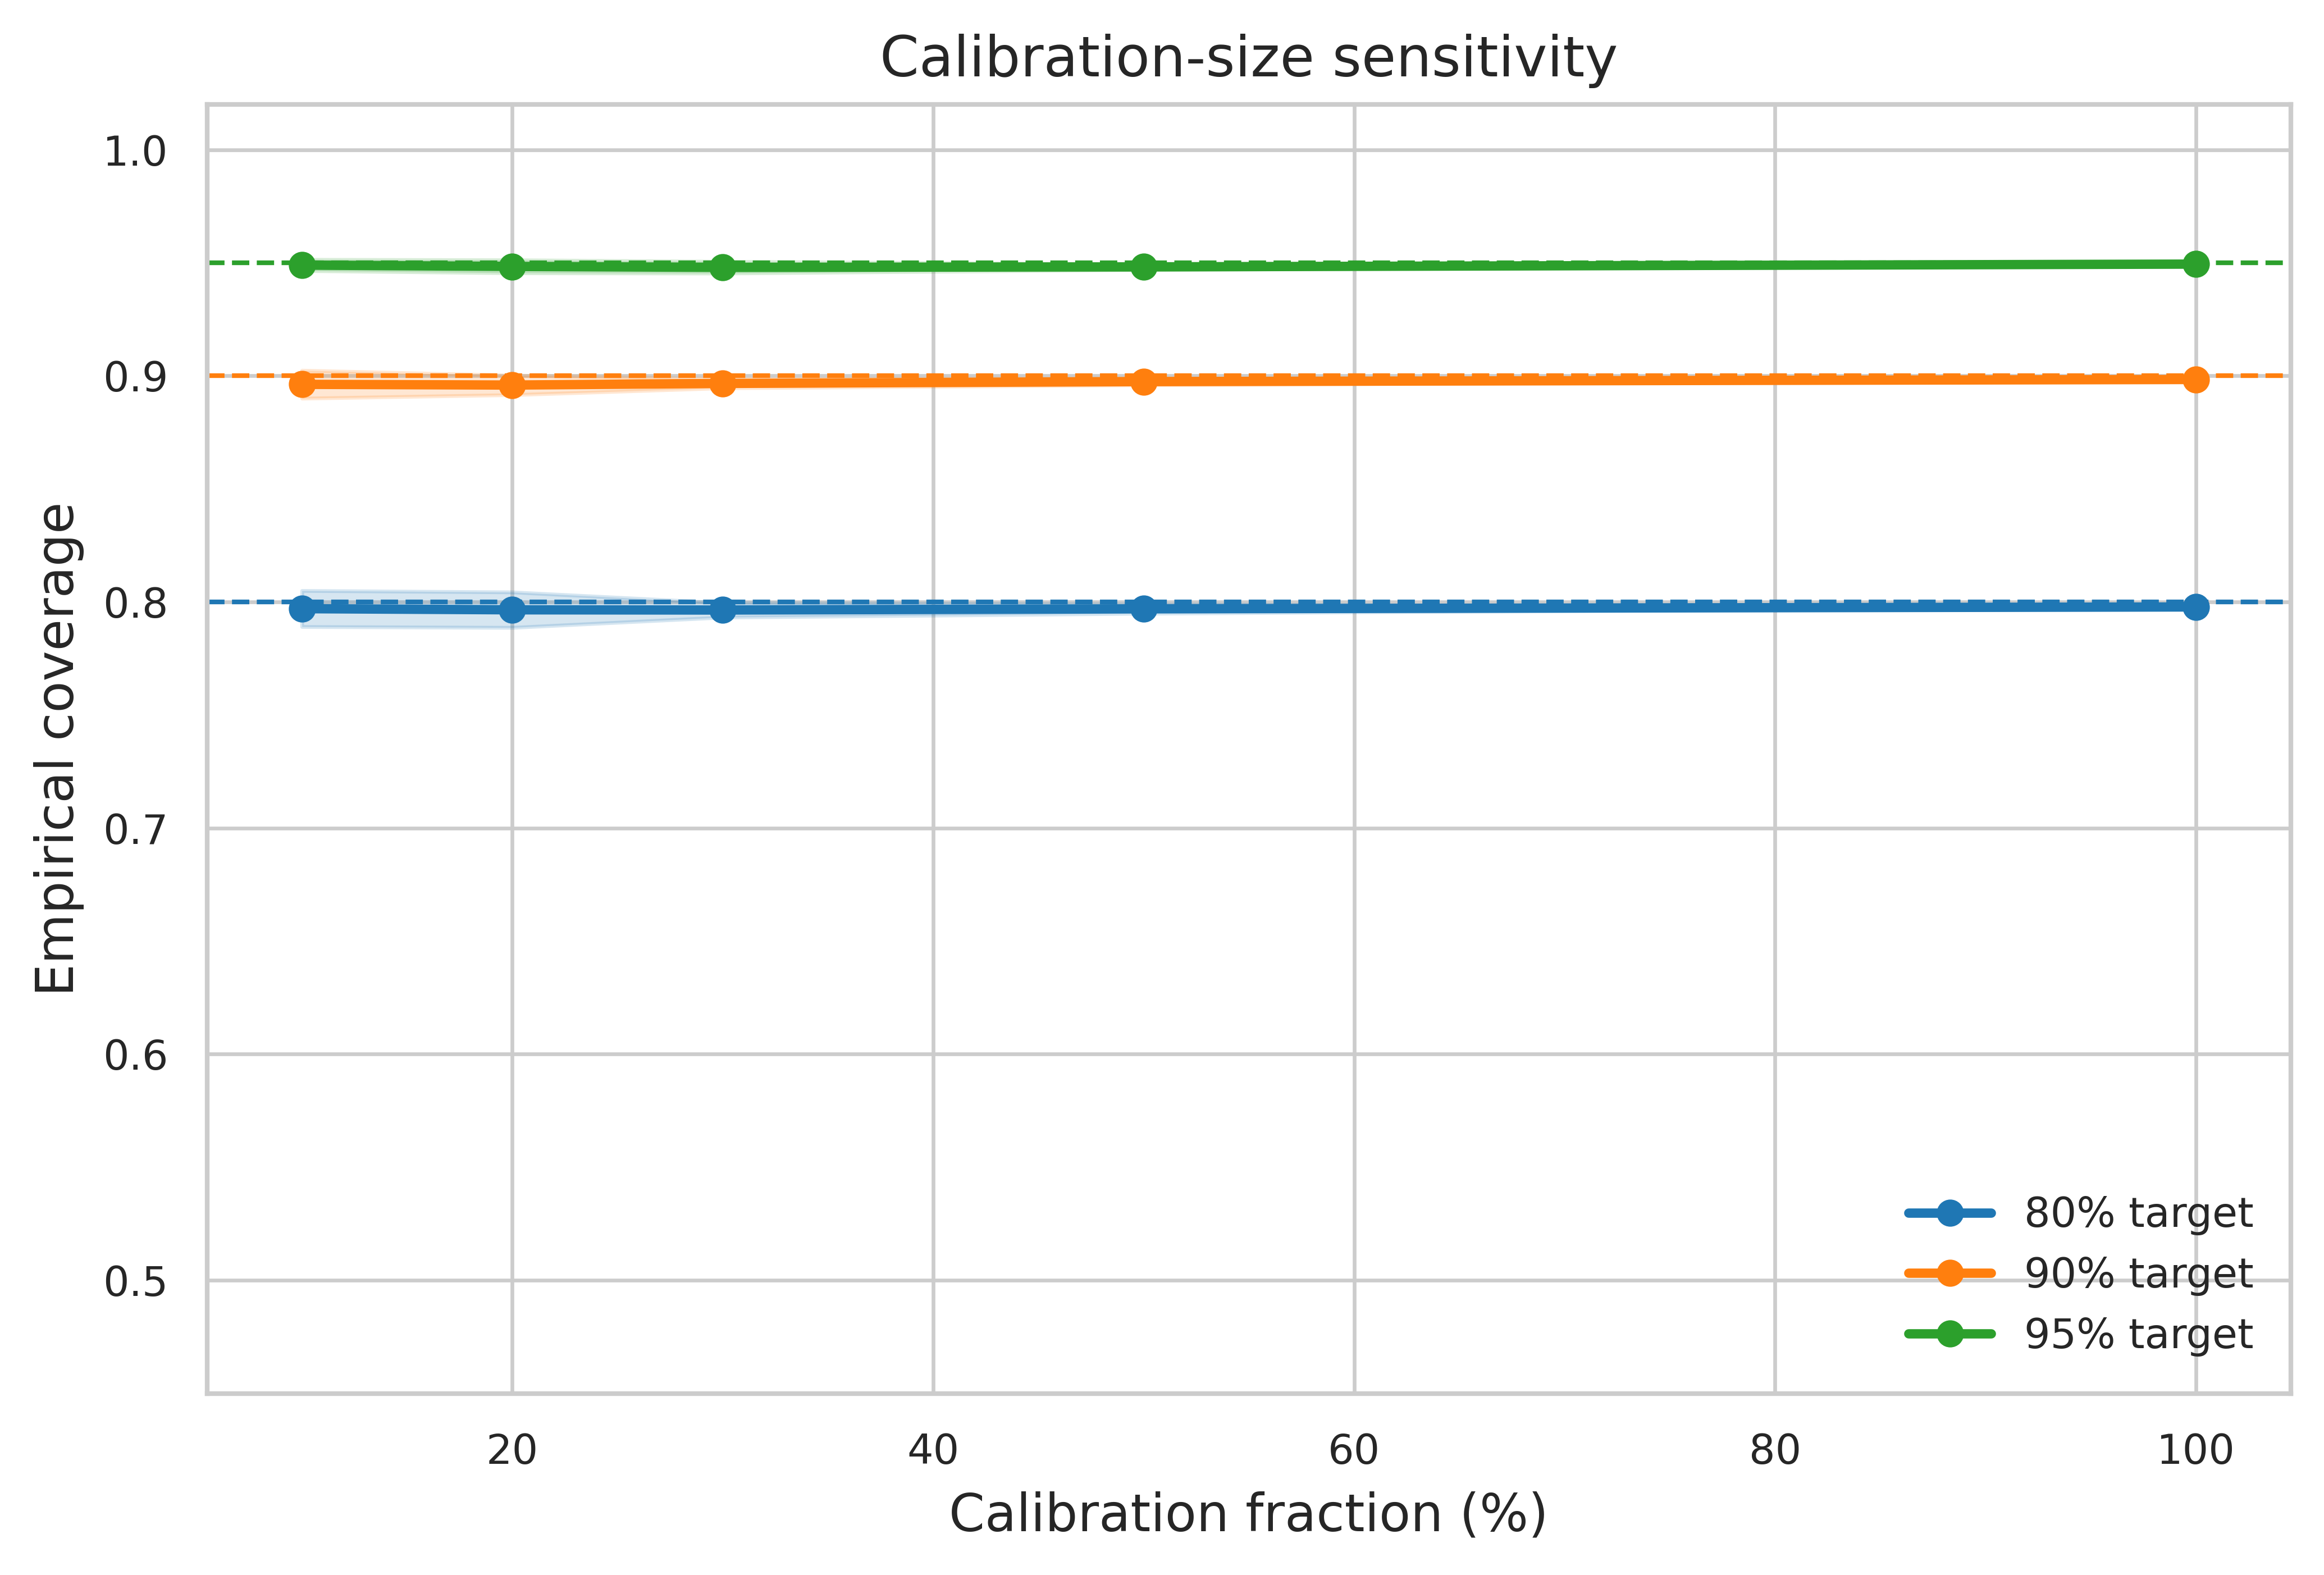
\includegraphics[width=\columnwidth]{figures/figure_12_calibration_size_sensitivity_original_prevalence.png}
\caption{Sensitivity of standard split-conformal marginal coverage to calibration-set size. Lines show means across ten stratified subsamples; shaded regions show one standard deviation.}
\label{fig:calsize}
\end{figure}

\subsection{Interpretability and subgroup results}
Permutation importance ranked HbA1c level (mean ROC-AUC decrease 0.1454) and blood glucose level (0.0954) as the dominant predictors, followed by age (0.0188) and BMI (0.0064). SHAP analysis showed the same leading variables (Fig.~\ref{fig:importance}). These associations should not be interpreted causally.

\begin{figure*}[t]
\centering
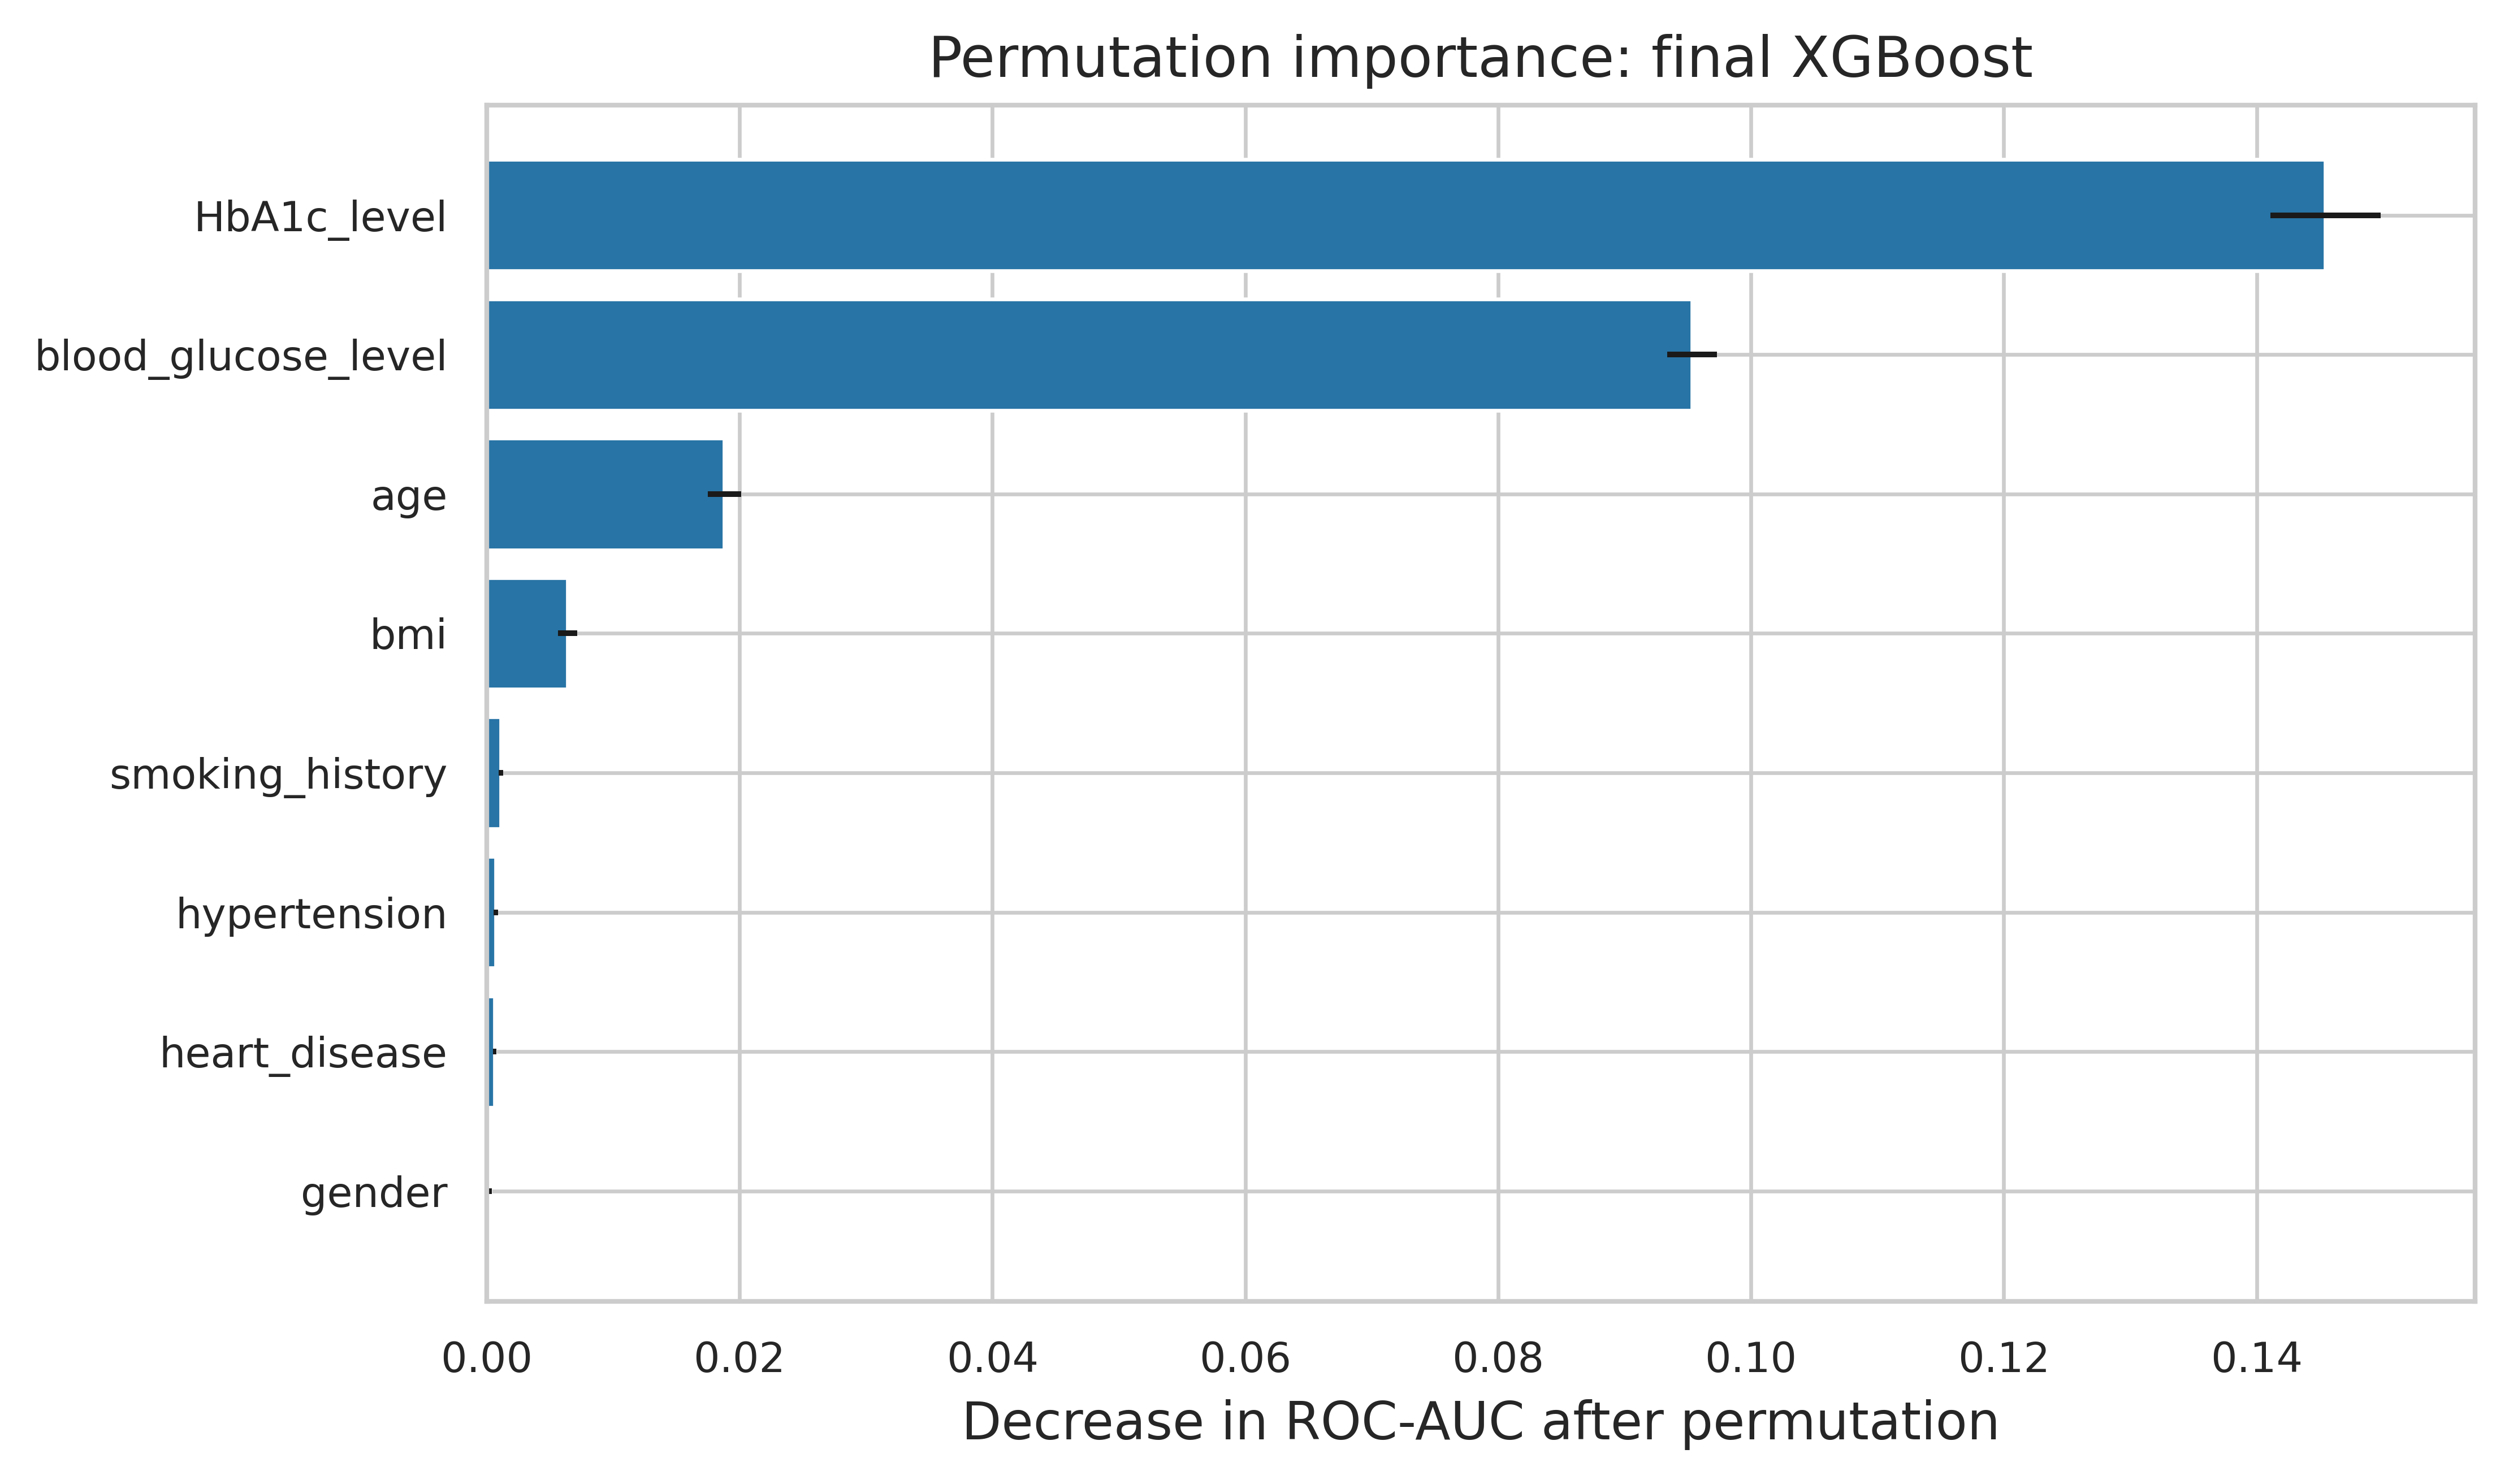
\includegraphics[width=0.48\textwidth]{figures/figure_13_permutation_importance_original_prevalence.png}
\hfill
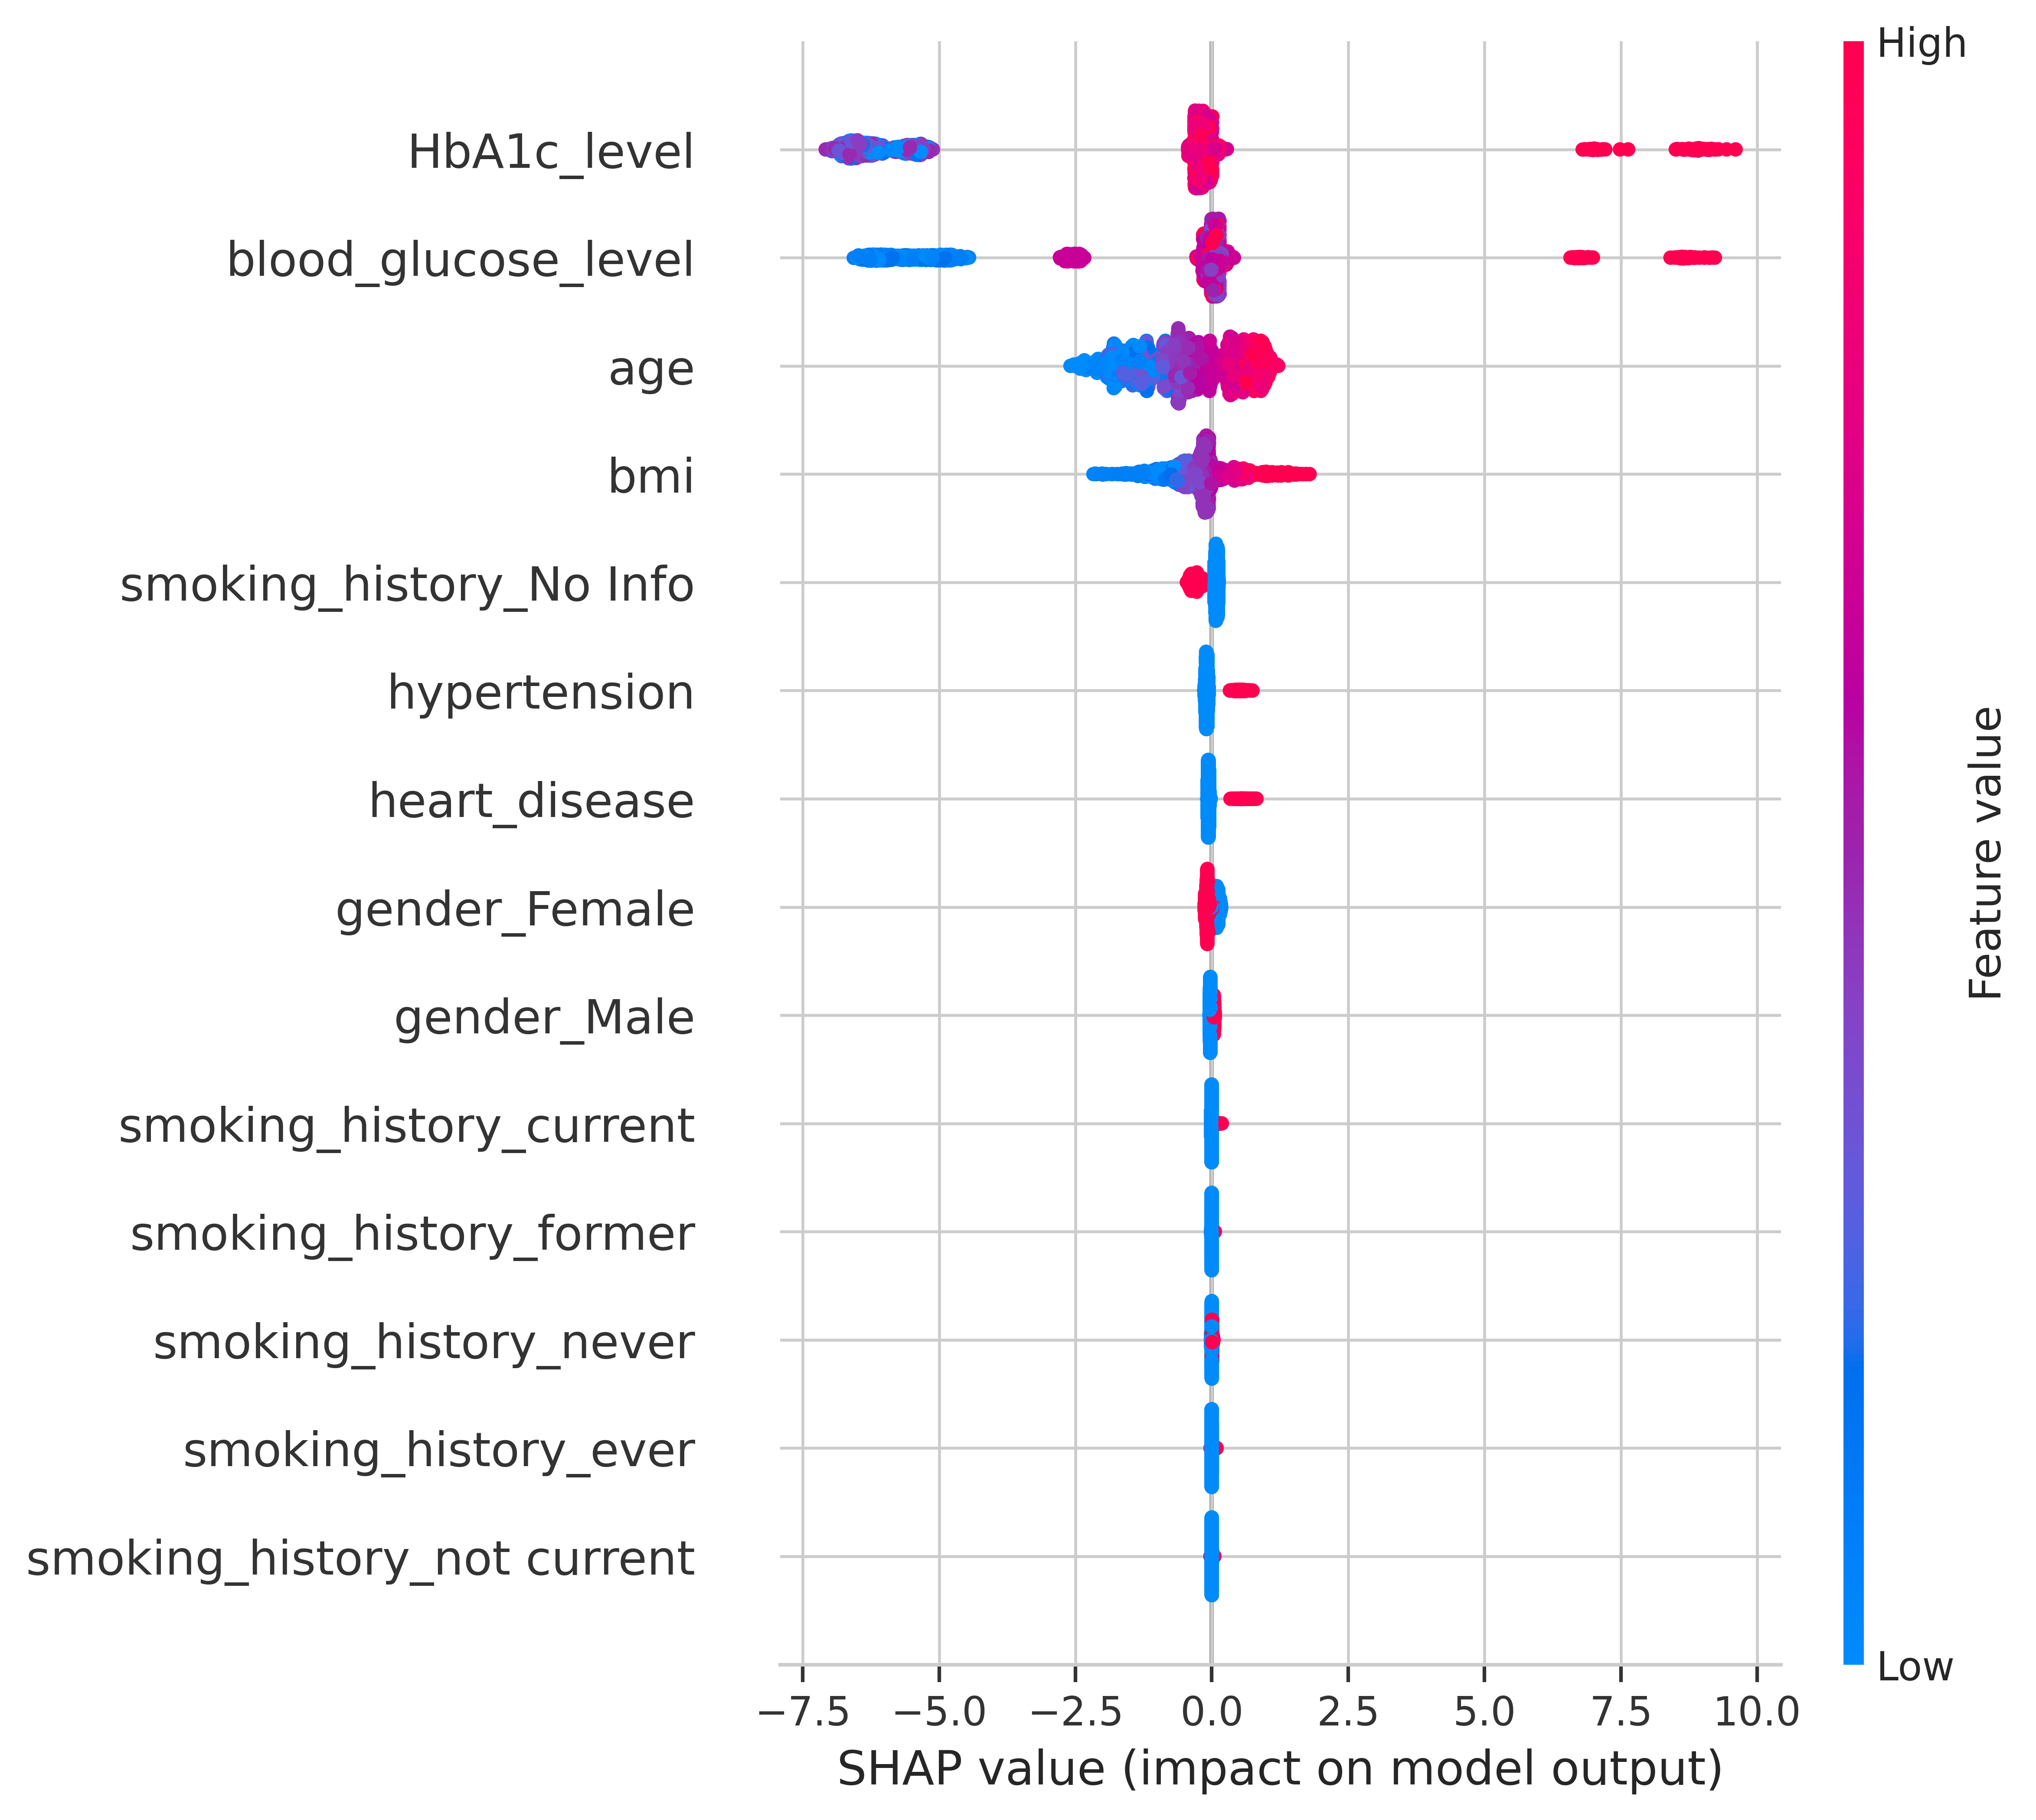
\includegraphics[width=0.48\textwidth]{figures/figure_14_shap_summary_original_prevalence.png}
\caption{Global feature-importance summaries for the fitted underlying XGBoost model. Left: permutation importance using test-set ROC-AUC. Right: SHAP summary plot.}
\label{fig:importance}
\end{figure*}

Point-prediction performance varied across observed subgroups. For example, sensitivity at threshold 0.5 was 0.7157 for female records and 0.7224 for male records. Sensitivity was 0.7441 among records aged 60 years or older and 0.7839 among records with hypertension. Standard conformal coverage also varied by subgroup; at 90\% confidence, coverage was 0.7365 among records aged 60 years or older and 0.6797 among records with hypertension. Mondrian conformal prediction improves class-conditional coverage overall but does not itself guarantee group-conditional coverage. Full subgroup tables and the corresponding figure are supplied in the reproducibility package.

\begin{figure}[t]
\centering
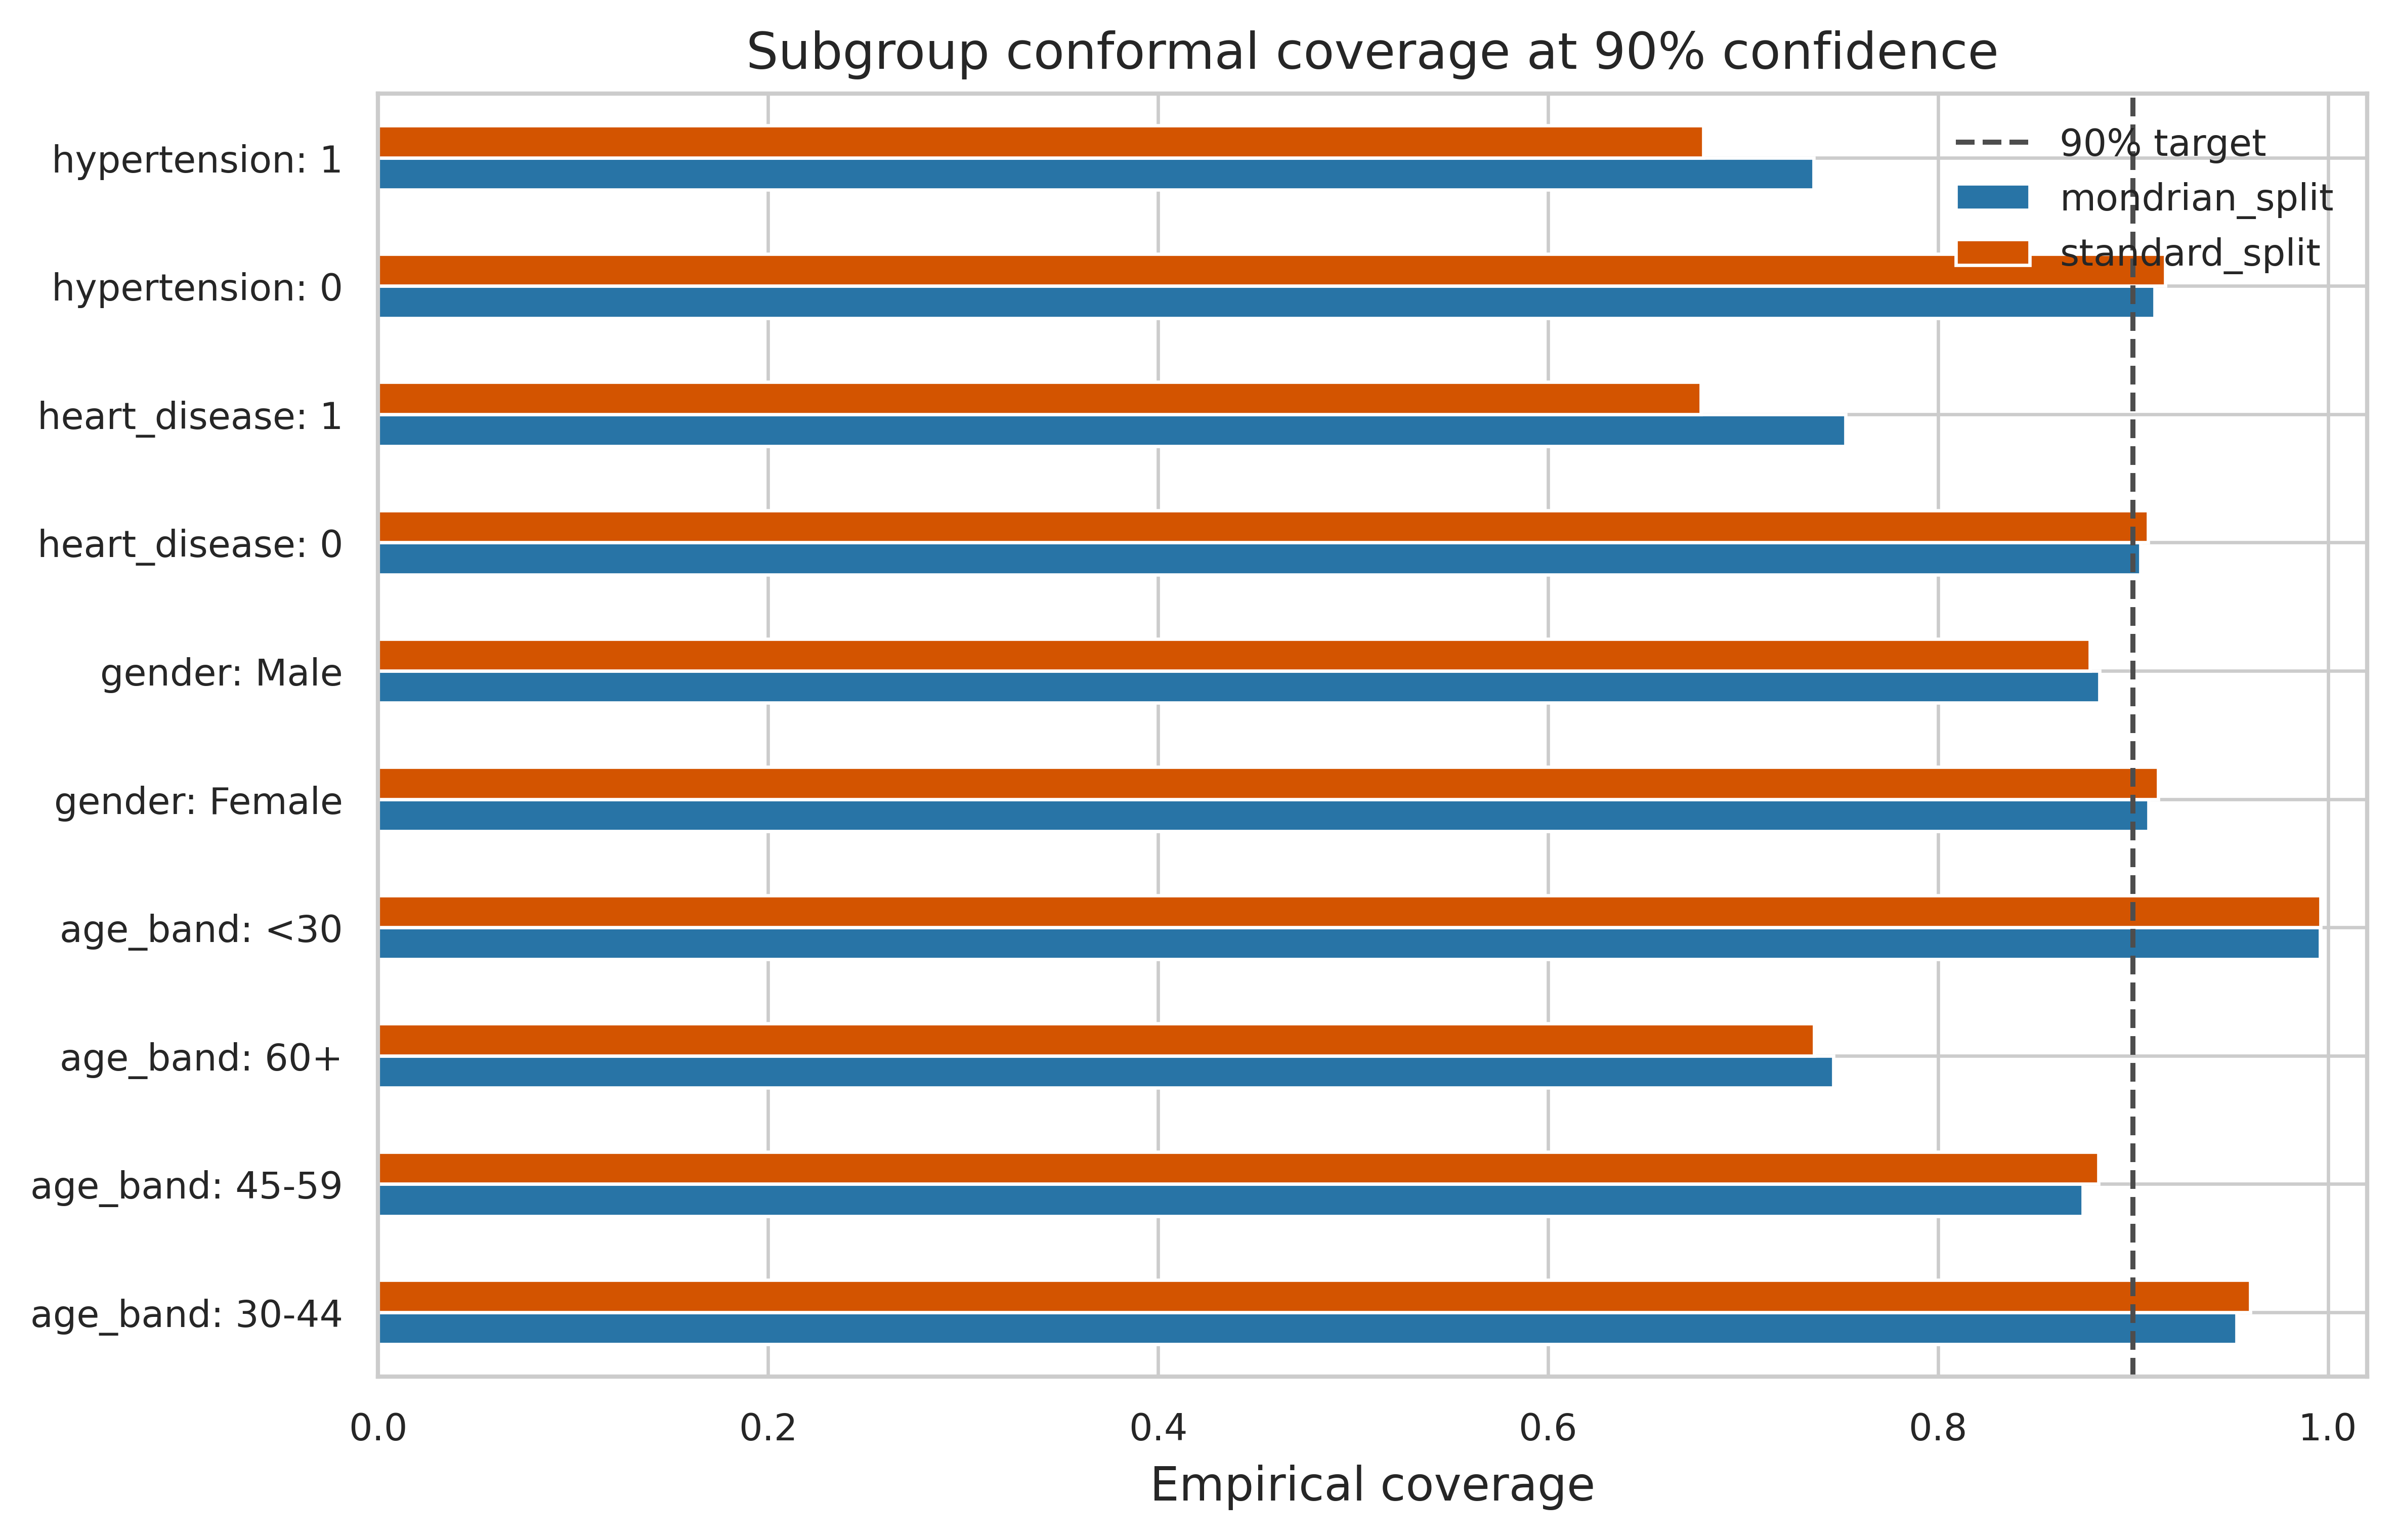
\includegraphics[width=\columnwidth]{figures/figure_18_subgroup_conformal_coverage_original_prevalence.png}
\caption{Observed subgroup coverage at 90\% confidence. These descriptive analyses do not establish group-conditional guarantees.}
\label{fig:subgroups}
\end{figure}

\subsection{Balanced sensitivity analysis}
An under-sampled balanced dataset was analyzed separately and is not used for the primary claims. It contained 16,964 records after cleaning, with 8,482 records in each class. On its balanced test set, XGBoost achieved accuracy 0.9045, balanced accuracy 0.9045, sensitivity 0.9092, specificity 0.8998, F1-score 0.9049, ROC-AUC 0.9767, and PR-AUC 0.9778. These values are not directly comparable to the primary prevalence-preserving results because the class distribution was intentionally altered.

\subsection{Secondary benchmark analysis using the Pima dataset}
A secondary benchmark analysis was conducted using the Pima Indians Diabetes Database, comprising 768 adult women of Pima Indian heritage and eight clinical predictors. The dataset contained 268 diabetes-positive records (34.9\%). Zero values in glucose, blood pressure, skin thickness, insulin, and BMI were treated as unavailable physiological measurements and were converted to missing values before split-safe imputation. On the Pima test partition, calibrated XGBoost achieved ROC-AUC 0.8211 (95\% CI, 0.7468--0.8839) and PR-AUC 0.7125 (95\% CI, 0.6174--0.8122). At the default threshold, sensitivity was 0.5370 and specificity was 0.8500. A training-selected threshold targeting 95\% sensitivity achieved test sensitivity of 0.9630, with specificity decreasing to 0.4400. Logistic regression and SVM showed slightly higher cross-validated ROC-AUC values than XGBoost in this small benchmark. Standard conformal prediction showed unstable class-wise coverage; Mondrian conformal prediction improved class-0 and class-1 coverage to 0.870 and 0.907 at nominal 90\% confidence. Because the test partition contained 154 records and 54 positive cases, uncertainty intervals were wide. The Pima results are therefore interpreted as a secondary benchmark of workflow reproducibility, rather than direct external validation of the primary model.

\subsection{External transportability evaluation in NHANES}
The external NHANES cohort contained 2,291 eligible adults, including 403 participants with self-reported clinician-diagnosed diabetes (17.59\%). Only the reduced harmonized model with sex, age, BMI, HbA1c, and fasting glucose was evaluated. It is therefore not a validation of the full primary eight-feature model. External discrimination remained strong: unweighted ROC-AUC was 0.9326 (95\% CI, 0.9186--0.9461) and PR-AUC was 0.7708 (95\% CI, 0.7303--0.8168). Calibration degraded externally: the Brier score increased from 0.0256 on the internal reduced-model source test set to 0.0811 in NHANES. Survey-weighted sensitivity analysis yielded ROC-AUC 0.9571, PR-AUC 0.8154, and Brier score 0.0505.

\begin{table*}[t]
\caption{Performance of the harmonized reduced calibrated XGBoost model internally and in the external NHANES cohort. NHANES results are unweighted primary transportability results.}
\label{tab:externalperformance}
\centering
\begin{tabular}{lrrrrrrrr}
\toprule
Evaluation cohort & $n$ & Prevalence & Sensitivity & Specificity & F1-score & ROC-AUC & PR-AUC & Brier score \\
\midrule
Source internal reduced-model test set & 19,226 & 8.82\% & 0.7134 & 0.9942 & 0.8048 & 0.9762 & 0.8765 & 0.0256 \\
NHANES external cohort & 2,291 & 17.59\% & 0.6055 & 0.9772 & 0.7072 & 0.9326 & 0.7708 & 0.0811 \\
\bottomrule
\end{tabular}
\end{table*}

Source-selected operating thresholds did not preserve their intended sensitivity targets externally. The threshold selected to target 95\% sensitivity using source training data achieved only 0.7246 sensitivity in NHANES, despite a low threshold of 0.0254. This result demonstrates that decision thresholds selected in one population should not be assumed to retain their operating characteristics in another population.

\begin{table}[t]
\caption{External performance of source-selected operating thresholds in NHANES.}
\label{tab:externalthresholds}
\centering
\begin{tabular}{lrrrr}
\toprule
Source target & Threshold & Sensitivity & Specificity & False negatives \\
\midrule
Default & 0.5000 & 0.6055 & 0.9772 & 159 \\
85\% sensitivity & 0.0800 & 0.6824 & 0.9682 & 128 \\
90\% sensitivity & 0.0490 & 0.6998 & 0.9645 & 121 \\
95\% sensitivity & 0.0254 & 0.7246 & 0.9576 & 111 \\
\bottomrule
\end{tabular}
\end{table}

Source-calibrated conformal thresholds did not retain nominal coverage in NHANES. At nominal 90\% confidence, standard split conformal prediction covered 52.36\% of diabetes-positive records. Mondrian conformal prediction improved diabetes-class coverage to 70.22\%, but it also remained below nominal coverage. At nominal 95\% confidence, Mondrian class-1 coverage was 72.70\%. These findings are consistent with a lack of exchangeability between source calibration data and the external cohort.

\begin{figure*}[t]
\centering
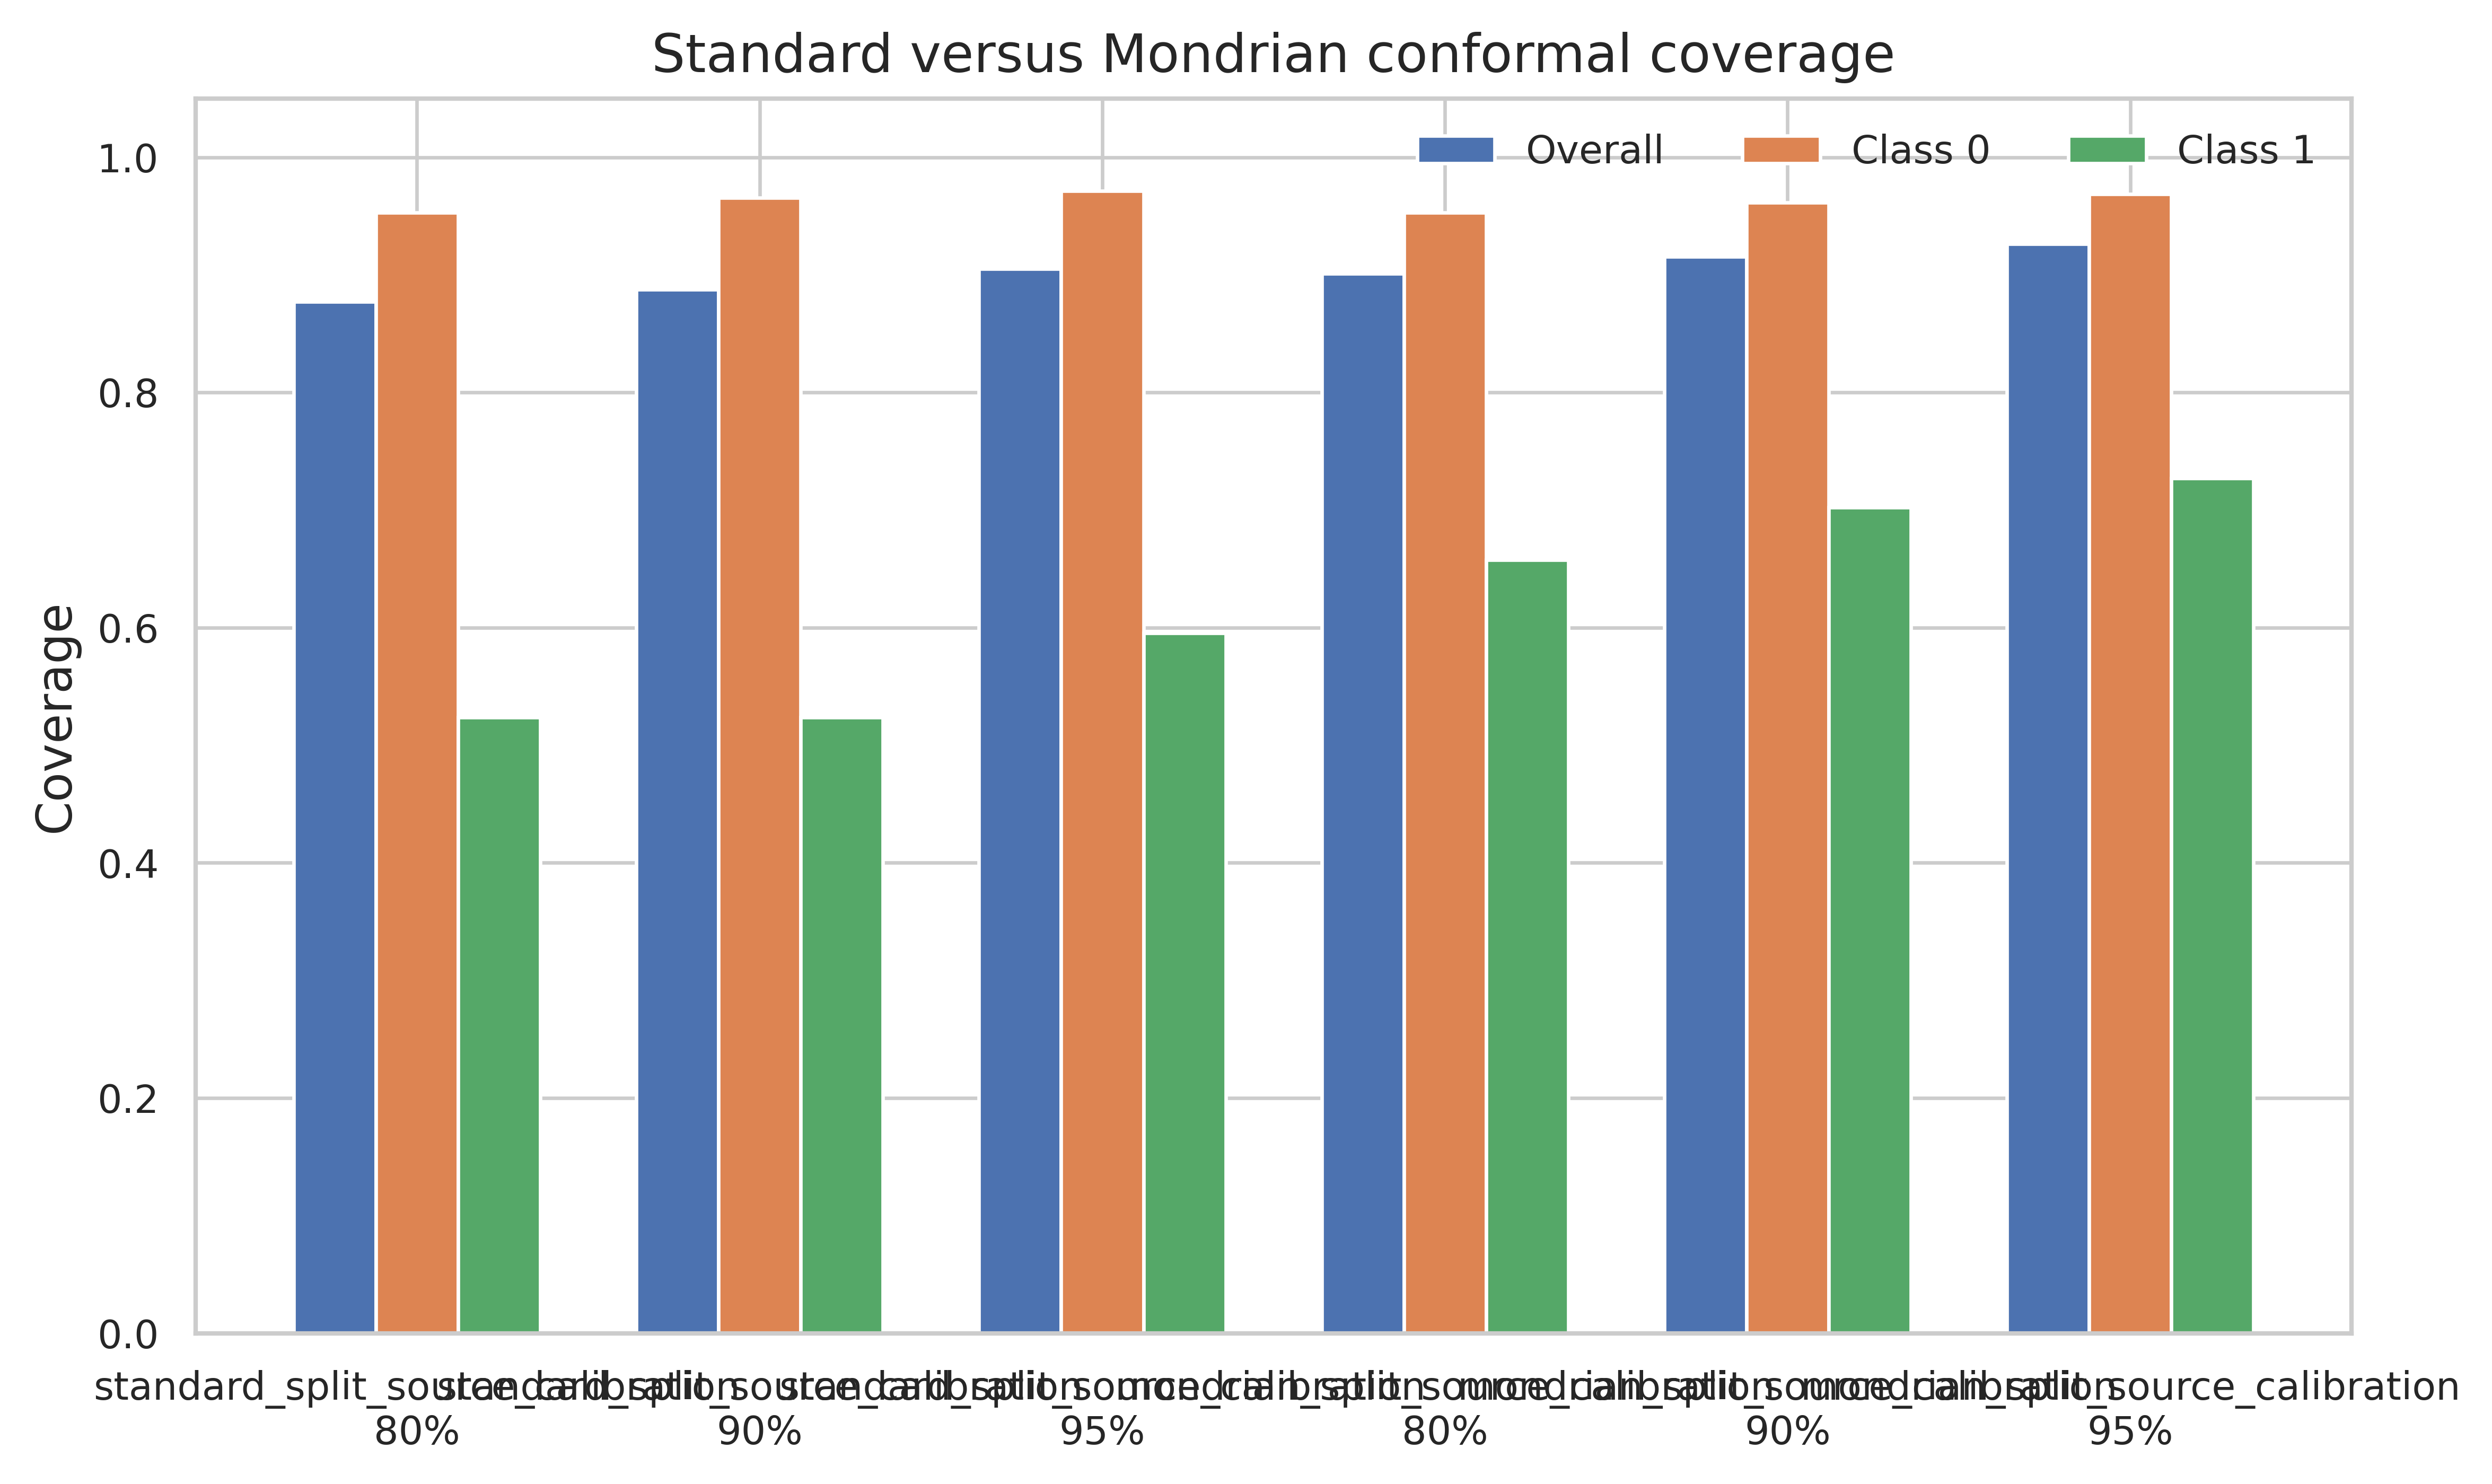
\includegraphics[width=0.78\textwidth]{figures/figure_nh02_external_conformal_method_comparison.png}
\caption{External NHANES conformal coverage using source-calibrated thresholds. Neither standard nor Mondrian conformal prediction retained nominal diabetes-class coverage after transport.}
\label{fig:externalconformal}
\end{figure*}

\begin{table*}[t]
\caption{External conformal coverage in NHANES using thresholds calibrated only on the source calibration partition.}
\label{tab:externalconformal}
\centering
\begin{tabular}{llrrrrr}
\toprule
Method & Confidence & Overall coverage & Class-0 coverage & Class-1 coverage & Mean set size & Empty-set rate \\
\midrule
Standard split & 90\% & 0.8878 & 0.9656 & 0.5236 & 0.9555 & 0.0445 \\
Standard split & 95\% & 0.9053 & 0.9714 & 0.5955 & 0.9847 & 0.0153 \\
Mondrian split & 90\% & 0.9158 & 0.9613 & 0.7022 & 0.9974 & 0.0026 \\
Mondrian split & 95\% & 0.9262 & 0.9688 & 0.7270 & 1.0183 & 0.0000 \\
\bottomrule
\end{tabular}
\end{table*}

\section{Discussion}
The reproducible workflow demonstrated strong discrimination for diabetes-status classification on the supplied public dataset. Importantly, the evaluation separates point-prediction performance from uncertainty quantification. The high default-threshold specificity was accompanied by sensitivity of 0.7188, showing that accuracy alone would have obscured a clinically important number of false negatives. The training-only threshold analysis demonstrated the expected trade-off: sensitivity increased when the classification threshold was lowered, while specificity and positive predictive value declined.

The comparison of conformal methods provides the central reliability result. Standard split conformal prediction met the intended marginal coverage targets but under-covered diabetes-positive observations. Mondrian conformal prediction produced near-nominal class-wise coverage at 90\% and 95\% confidence, at the cost of broader prediction sets. This is an appropriate trade-off for uncertainty-aware reporting: a doubleton set communicates ambiguity directly, whereas a forced singleton label would conceal it. Clinical use would require a predefined policy for handling singleton, doubleton, and empty sets.

The external NHANES results demonstrate that discrimination can remain strong while probability calibration, operating thresholds, and conformal coverage do not fully transport. Source calibration did not maintain nominal diabetes-class conformal coverage in the external cohort. This evidence is consistent with a violation of the exchangeability assumption between source calibration data and the target population; conformal prediction is not a substitute for target-domain validation.

Several limitations constrain interpretation. The external evaluation used a reduced five-feature model because only those variables could be harmonized; it does not validate the complete primary eight-feature model. The NHANES outcome was self-reported clinician-diagnosed diabetes and therefore differs from the source outcome. HbA1c and blood glucose are closely connected to diabetes assessment, so the results should not be interpreted as evidence of early prediction before clinical testing. Pima was a small secondary benchmark in a distinct population, not direct external validation. Subgroup analyses were descriptive and cannot establish fairness or causal mechanisms.

Future work should recalibrate probabilities, operating thresholds, and conformal scores using representative labelled target-domain data; assess clinical decision consequences; and perform prospective evaluation before any deployment claim. The present results support a transparent analytical framework, not autonomous clinical decision making.

\section{Conclusion}
Calibrated XGBoost combined with class-conditional conformal prediction provided strong internal discrimination and transparent uncertainty reporting on a prevalence-preserving public diabetes-status dataset. Standard split conformal prediction was insufficient for internal class-wise reliability, whereas Mondrian conformal prediction achieved near-nominal internal class-0 and class-1 coverage at the cost of more informative multi-label prediction sets. External NHANES evaluation retained strong discrimination but showed degraded calibration, non-transportable source-selected thresholds, and below-nominal diabetes-class conformal coverage. The complete workflow provides a reproducible basis for target-domain recalibration and prospective validation; it does not justify direct clinical deployment without those steps.

\section*{Data Availability}
The source dataset is publicly available from Kaggle \cite{mustafa2023dataset}. The NHANES external cohort can be reconstructed from the public 2017--2018 NHANES files \cite{nhanes2018overview,nhanes2018glu}. The cleaned datasets and train/calibration/test partitions can be regenerated using the supplied pipeline, subject to the applicable source-data licenses.

\section*{Code Availability}
The reproducibility code, environment specification, run instructions, and high-performance computing scripts are available at \url{https://github.com/diwakardkk/Confirmal_Prediction}. The repository should be updated to the final tagged analysis commit before manuscript submission.

\section*{Ethics Statement}
The analysis used a public secondary dataset and did not involve interaction with human participants or access to direct identifiers. Institutional and publisher-specific requirements for secondary-data research should be confirmed by the authors before submission.

\section*{Conflict of Interest}
The authors declare no conflict of interest.

\section*{Funding}
Replace with funding information or state: ``This research received no external funding.''

\appendices
\section{Reproducibility Artefacts}
The accompanying \texttt{results/} directory contains the generated CSV and XLSX tables used to prepare the manuscript. The \texttt{figures/} directory contains 600-dpi PNG figures. The main analysis command is documented in the project README.

\bibliographystyle{IEEEtran}
\bibliography{ref}

\end{document}
